% !TEX root = ./diss.tex

\chapter{Experiment 2}

The goal of Experiment~2 was to replicate and extend Experiment~1 in an attempt to answer some remaining questions about the spacing effect.  We examined patterns of effects across short, medium, and long lags to determine whether these spacing effects are modulated by these parameters.  For example, deficient processing may still be present at shorter lags (this is important to scrutinize due to its status as an ``impostor effect''; \citeNP{DelaEtal2010}), there may be differences in reinstatement (study-phase retrieval) at longer lags, or we may see other effects change in a graded fashion.  Graded effects would qualify more specifically as a lag effect \cite{Gree1989a,KahaHowa2005}, showing that long-term memory improves as spacing increases.
The presence of these gradations would allow us to better interpret data patterns that fit multiple theories.  Experiment~1 used lags of 0 and 12; this experiment keeps these lags and adds repetitions at lags of 2 and 32, which are within the range of lags from behavioral spacing studies.

We expected that memory performance would show a lag effect: subsequent memory will correlate positively with lag.  The most informative EEG effects regarding the spacing effect in Experiment~1 were for the N1, upper alpha, and time--frequency similarity, though the latter were difficult to interpret.  Overall, they implicate differences in attention and semantic processing between spaced and massed repetitions that led to interactions with subsequent memory.  It will be important to examine whether these effects modulate with additional lags.

We also included single-presentation stimuli at test, which allowed us to get a baseline measurement of memory performance for comparison of subsequently remembered and forgotten massed and spaced items.  We expected a repetition effect (repeated items will be remembered better than single presentation items), but perhaps if massed repetitions do involve deficient processing then they will be recalled no better than single presentation items.

\section{Method}

\subsection{Participants}

% subNum = [1,2,3,4,5,6,7,8,9,10,11,12,13,14,15,16,17,18,19,20,21,22,23,24,25,26,27,28,29,30,31,32,33,34,35,36,37,38,39,40];
% age = [20, 18, 20, 18, 25, 18, 18, 26, 19, 18, 22, 19, 18, 22, 25, 25, 19, 19, 19, 18, 29, 20, 25, 18, 22, 21, 20, 23, 22, 22, 24, 20, 22, 24, 21, 23, 26, 21, 23, 20];
% gender = [1, 2, 2, 2, 2, 2, 2, 1, 1, 2, 2, 2, 1, 1, 1, 1, 1, 1, 1, 2, 1, 2, 2, 1, 1, 2, 2, 1, 2, 1, 2, 2, 1, 2, 1, 1, 1, 2, 1, 1]; % (1 = male, 2 = female)
% excludedSub = [];
% % excludedSub = [2,3,9,13,20,23,24,27,39,7,16,25,34];
% numSub = sum(~ismember(subNum,excludedSub))
% mean(age(~ismember(subNum,excludedSub)))
% min(age(~ismember(subNum,excludedSub)))
% max(age(~ismember(subNum,excludedSub)))
% sum(gender(~ismember(subNum,excludedSub)) == 2) % females

Forty University of Colorado Boulder undergraduates participated in the experiment for payment of \$15 per hour (ages 18--29, $M=21.3$; 19 female).  All participants were right-handed native-English speakers and had normal or corrected-to-normal vision.  Informed consent was obtained from each participant, and the study conformed to the Institutional Review Board guidelines.

\subsection{Materials}

The stimuli and experiment presentation software were the same as for Experiment~1.

\subsection{Design}

%(Figure~\ref{fig:space2_exp})

Experiment~2 consisted of two sessions, each of which had nine blocks of three experimental phases: study, distractor, test.
\cbstart
Two sessions were used to gather enough trials across the additional conditions.
\cbend
The phases were similar to Experiment~1 (Figure~\ref{fig:space_exp}, page~\pageref{fig:space_exp}).  The phase differences were that the exposure phase was excluded to keep the experiment length reasonable and there was no recognition test.
% Since the exposure phase was also to be used for classification, we decided that didn't need to be run for Exp~2.
The sessions, including application of the electrode net and running in the task, lasted approximately 2.5 hours.  Stimuli were randomly shuffled prior to creating the list for each phase at the beginning of the first session.  The study phase contained the conditions that were manipulated within subjects, namely the viewing of spaced and massed paired associates.

\subsection{Procedure}

An electrode net was applied to each participant's head, and the first session began with a shortened practice version of the experiment to familiarize participants with the study and test procedures.

% \begin{figure}
%   \centering
%   \begin{tabular}{l}
%   \includegraphics[width=.9\textwidth]{./figs/exp2/space2_example_study_fix} \\
%   \includegraphics[width=.7\textwidth]{./figs/exp2/space2_example_test}
%   \end{tabular}
%   \caption{Experiment~2: Study and test phases}
%   \label{fig:space2_exp}
%   %\ref{fig:space2_exp}
%   %\pageref{fig:space2_exp}
% \end{figure}

% for each category, 3 image trials of each of 5 types: 

% (((9+3)*2)+3+2)*2

In each study phase block, participants viewed word--image pairs and were asked to think of a relationship between them or to make up a story pairing them.  They were told that a subsequent test would require them to remember the word associated with each picture, but they were not told that some pairs will repeat.  Spaced items were presented at a lag of either 2, 12, or 32, and massed items were presented at a lag of zero.  For each of the two image categories there were three two-presentation spaced pairs per lag, three two-presentation massed pairs, three pairs presented only once, and four additional single-presentation buffers (two at the beginning of the list and two at the end).  Buffer pairs did not appear on the test list.
% All images (including spaced, massed, and single presentation items) were included on the test list.
Thus, there were 58 word--image presentations in each block.  On each trial, a fixation cross appeared for 1.0--1.2~s (jittered), then the word was presented first for 1.0~s followed immediately by the image for 1.0~s.  No more than three images from the same category could occur in a row, and no more than two trials with the same lag (including single-presentation pairs) could occur in a row.  Each study phase lasted approximately 3.5~min.

In the distractor phase, participants answered simple math problems of the format \texttt{A+B+C=?} for 2~min.  They typed their responses with the keyboard.  Different tones occurred for correct and incorrect answers, and mean accuracy and response time was reported to the participant at the end of the phase.

% \begin{figure}
%   \centering
%   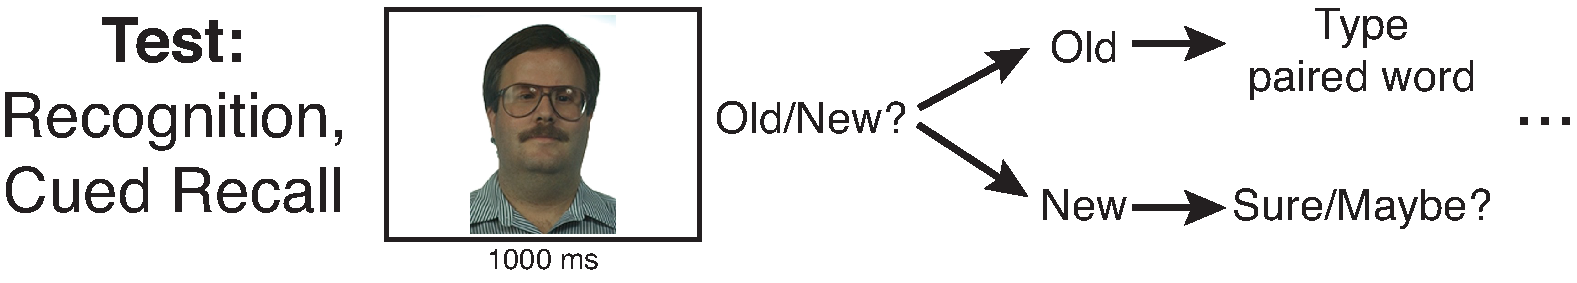
\includegraphics[width=\textwidth]{./figs/exp1/space_example_test}
%   \caption{Experiment~1: Test phase}
%   \label{fig:space_test}
%   %\ref{fig:space_test}
%   %\pageref{fig:space_test}
% \end{figure}

Finally, in the test phase, participants performed a cued recall task.  Thirty images (nine spaced, three massed, and three single presentation images from each category) were mixed together and presented one at a time.  Participants saw \texttt{???????} below each image and had to type the word previously paired with the image; they could pass if they could not remember the word.  On each trial, a fixation cross appeared for 1.0--1.2~s (jittered) and the image was shown for 1.0~s, at which point the question marks appeared and participants were asked to make their response.  Importantly, test images were presented in a sequence similar to the study order.  To construct the test list, the positions of the second presentations of study stimuli were divided into fifteen contiguous groups and each group was shuffled internally.  This was done to approximately preserve a similar amount of time between the second presentation and the test across all ``old'' stimuli.  Each test phase lasted approximately 3~min.

% 3.0~s timer for recognition and new responses

% There were approximately 7~min between studying a spaced or massed word--image pair and seeing that image on the test list.

\subsection{Electrophysiological recordings and data processing}

All procedures for recording and processing electrophysiological data was the same as in Experiment~1, as was finding ERP component peaks and analyzing ERP and time--frequency data.

\section{Results}

% DNF session 2:
% SPACE2003
% SPACE2009
% SPACE2013 % didn't record EEG so stopped in middle of session 1
% SPACE2020
% SPACE2023
% SPACE2024
% SPACE2027
% SPACE2039

% performance more than 2 STD below mean in some cases (e.g., lag 32):
% SPACE2007 (also rejected below)
% SPACE2025 (also rejected below)

% EEG trials < 10:
% SPACE2002 (also rejected below)
% SPACE2007 (also rejected above)
% SPACE2025 (also rejected above)
% SPACE2034

% noisy EEG:
% noisiest first: 2, 16, 22, 40, 26, 36, 10, 17; only rejecting 2 and 16
% SPACE2002 (also rejected above)
% SPACE2016

Ten participants were excluded from all analyses either because they did not return for the required second session ($n=8$) or their performance in important conditions was more than 2 standard deviations below the mean ($n=2$).  The remaining thirty participants were included in behavioral analyses.
Three additional participants were excluded from ERP and time--frequency analyses either because they had extremely noisy EEG ($n=2$) or had fewer than 10 artifact-free trials in any of the main trial conditions ($n=1$), leaving twenty-seven participants in EEG analyses.  Similarity analyses included the same participants, all of whom had six or more artifact-free pairs of initial presentation--repetition image trials.

All analyses contingent on subsequent memory are split by whether words were recalled or forgotten.  There was no recognition test as in Experiment~1 (during cued recall, all test stimuli were ``old''), so the ``forgotten'' trials category contained both images that were completely forgotten and those where participants were only unsure about the paired words.

\subsection{Behavioral results}

An ANOVA with factors of session (1 and 2), spacing (single presentation, massed/lag 0, short/lag 2, medium/lag 12, and long/lag 32 spaced), and image category, was run on cued recall hit rate.  There was a main effect of spacing [$F(4,116)=174.2, p=2.62e^{-36}$] in the expected order, clearly showing a lag effect: long spaced words ($M=56.9\%$) were recalled better than medium spaced words ($M=49.2\%$), and, in turn, performance for short spaced ($M=45.8\%$), massed ($M=35.7\%$), and single presentation words ($M=23.0\%$) was better than the next.  Words paired with faces and scenes were recalled at the same rate (faces: $M=44.0\%$; scenes: $M=40.2\%$).  Thus, there are again clear spacing effects that scale with lag, as well as a simple repetition effect. These rates are comparable to Experiment~1.

There were also session $\times$ image category [$F(1,29)=7.96, p<.01$] and spacing $\times$ image category [$F(4,116)=7.52, p<.0005$] interactions such that recall was better for faces in session 1 compared to session 2, and performance increased at the longest lag for faces compared to scenes.  However, these effects do not speak to our investigations of the spacing effect and will not be reported in detail.

Massed items were remembered significantly better than single-presentation items but less well than short (2) spaced items; this still leaves open the possibility that deficient processing occurs for massed items and decreases with lag.  Only 9.3~sec elapsed between a short spaced item's initial presentation and repetition, whereas the delay was 3.1~sec for massed items.  Neural effects can shed light onto how cognitive processes contribute to the spacing effect.  As there were no behavioral effects of session that interacted with spacing, EEG analyses were collapsed over the two sessions.

\subsection{ERP results}

ERP component peaks in Experiment~2 were at the same electrodes as in the previous experiment, but were slightly earlier in time.
%\hl{(Comment/question for Tim: I think latency difference is because for Exp~1 we didn't know about the EGI's A/D DIN delay so the correct offset (8~ms @ 250~Hz) was not used. Also, I used the average photocell offset for Exp~2 (17~ms) because tclab didn't want to deal with the photocell for every session, but I segmented to the actual photocell DINs for Exp~1. What should I do about this? The ``correct'' thing would be to redo Exp~1 analysis...)}
The visual N1 peaked at electrode~58 (T5) at $144$~ms (Figure~\ref{fig:s2_N1}; $\pm$50~ms window).  The N400 peaked at Cz at $352$~ms (Figure~\ref{fig:s2_N400}; $\pm$75~ms window used due a slight spreading of the peak voltage).  The LPC peaked at electrode~77 at $536$~ms (Figure~\ref{fig:s2_LPC}; $\pm$100~ms window).  Again, analyses use these peak electrodes and neighbors during study period words stimuli.  After examining condition grand averages, it seems that voltages were overall slightly attenuated compared to Experiment~1; it is hard to give a reason for this, but one possibility is that the electrode cap was placed in slightly different locations for Sessions~1 and 2.
% Again, during studied words the visual N1 peaked at $144$~ms (Figure~\ref{fig:s2_N1}), the N400 peaked at $352$~ms (Figure~\ref{fig:s2_N400}), and the LPC peaked at $536$~ms (Figure~\ref{fig:s2_LPC}).
Three-way ANOVAs with factors of spacing (massed and short, medium, and long spacing), presentation (1/new and 2/old), and subsequent memory (recalled and forgotten words) were performed on the averaged window voltages for word presentations.  Significant results are reported.

% \hl{How best to test single presentation items?}

% plot: N1 at E58 + surround
\begin{figure}[hp]
  \centering
  \begin{tabular}{cc}
  %Massed & Spaced-2 \\
  \multicolumn{1}{c}{(a) Massed} & \multicolumn{1}{c}{(b) Spaced-2} \\
  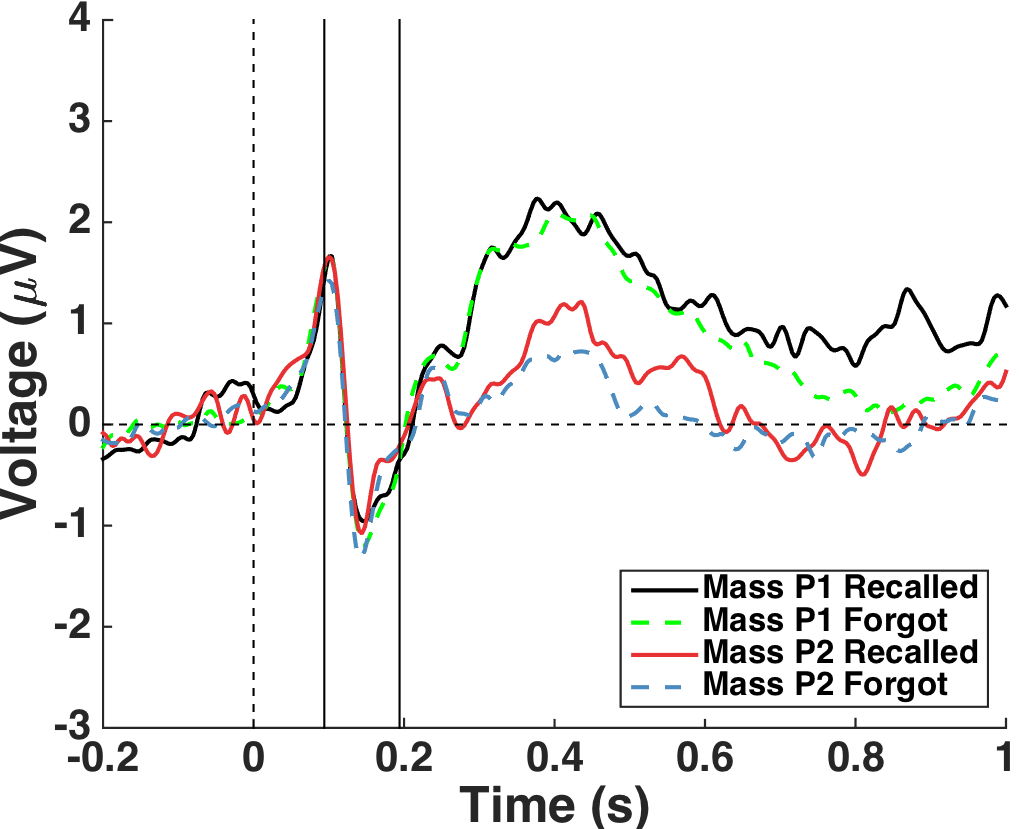
\includegraphics[width=.35\textwidth]{./figs/exp2/tla_single_ga_word_rc_mass_p1_word_fo_mass_p1_word_rc_mass_p2_word_fo_mass_p2_E50_E51_E57_E58_E59_E64_E65_-200_1000_legend_xylabel} &
  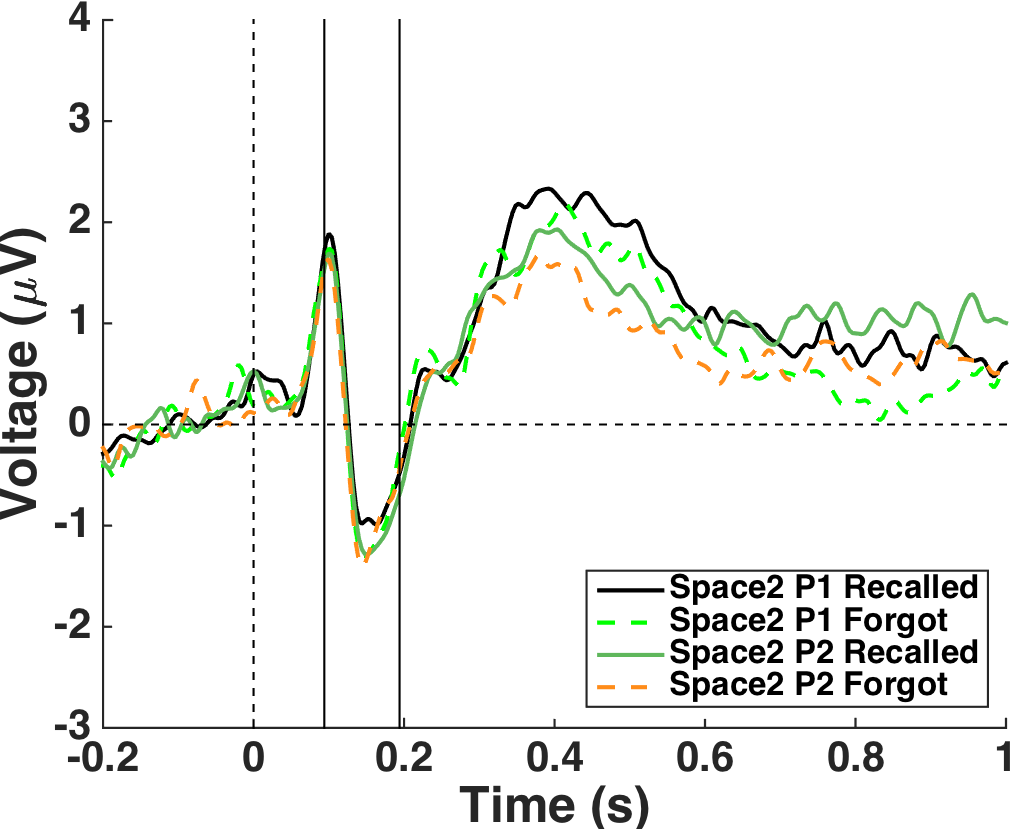
\includegraphics[width=.35\textwidth]{./figs/exp2/tla_single_ga_word_rc_spac2_p1_word_fo_spac2_p1_word_rc_spac2_p2_word_fo_spac2_p2_E50_E51_E57_E58_E59_E64_E65_-200_1000_legend_xylabel} \\
  %Spaced-12 & Spaced-32 \\
  \multicolumn{1}{c}{(c) Spaced-12} & \multicolumn{1}{c}{(d) Spaced-32} \\
  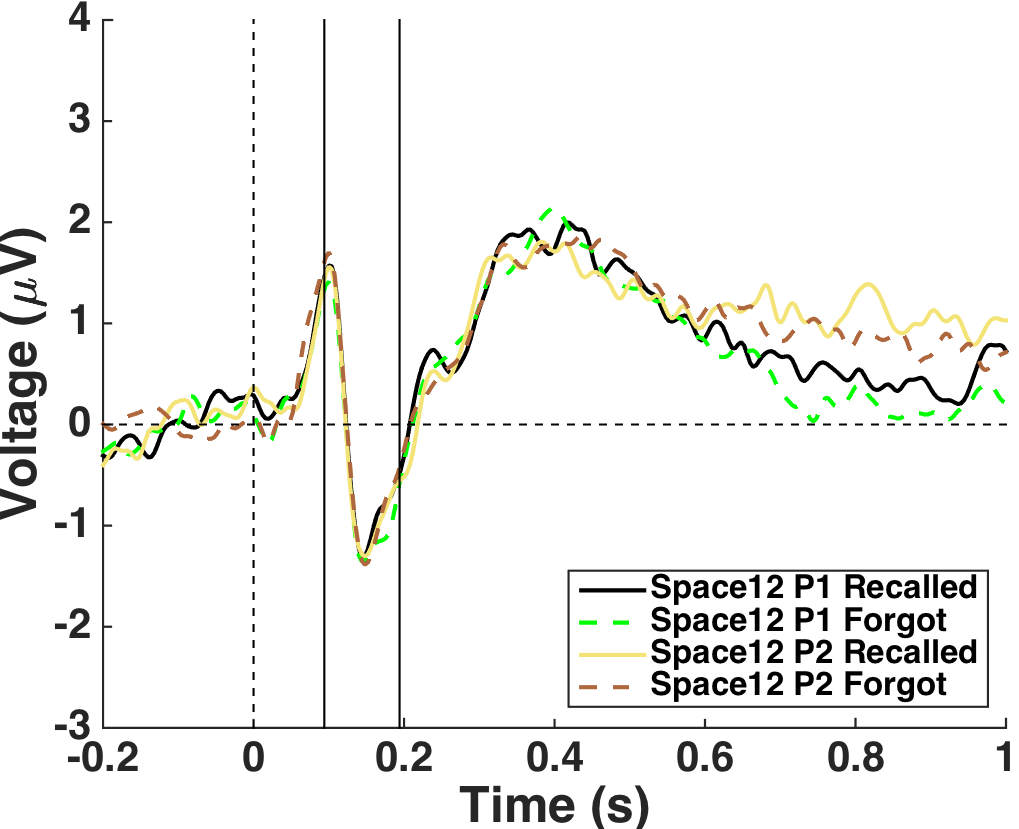
\includegraphics[width=.35\textwidth]{./figs/exp2/tla_single_ga_word_rc_spac12_p1_word_fo_spac12_p1_word_rc_spac12_p2_word_fo_spac12_p2_E50_E51_E57_E58_E59_E64_E65_-200_1000_legend_xylabel} &
  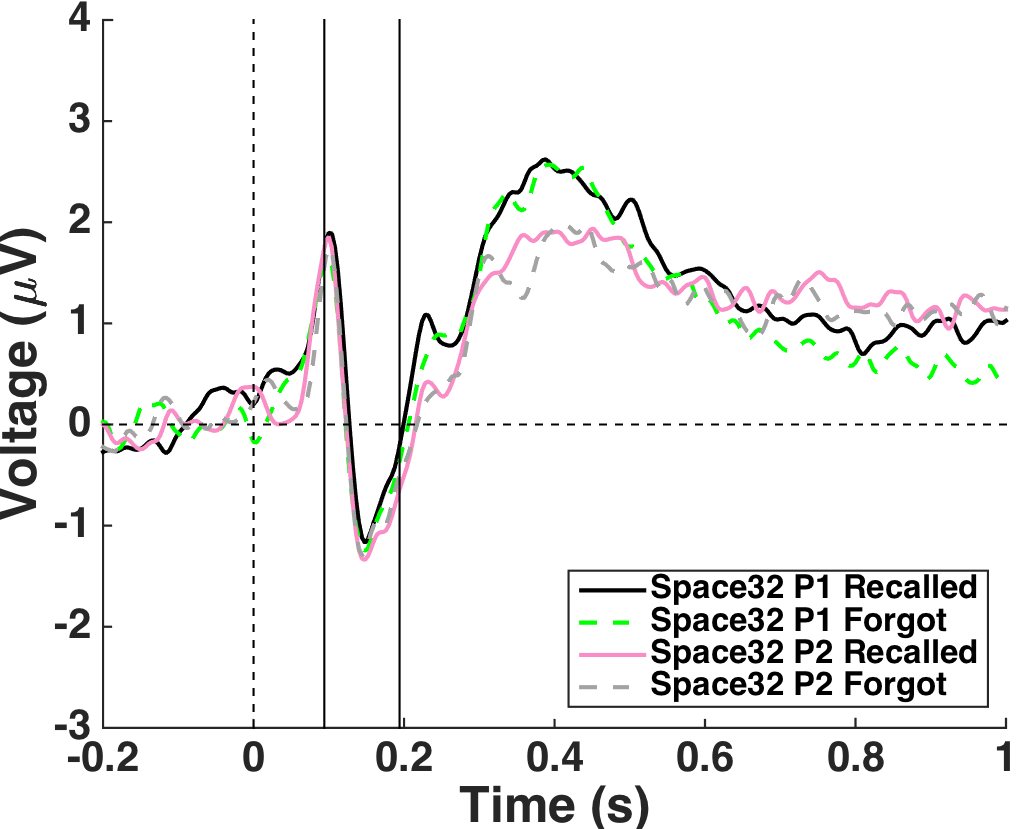
\includegraphics[width=.35\textwidth]{./figs/exp2/tla_single_ga_word_rc_spac32_p1_word_fo_spac32_p1_word_rc_spac32_p2_word_fo_spac32_p2_E50_E51_E57_E58_E59_E64_E65_-200_1000_legend_xylabel} \\
  \multicolumn{2}{c}{(e) Means} \\
  \multicolumn{2}{c}{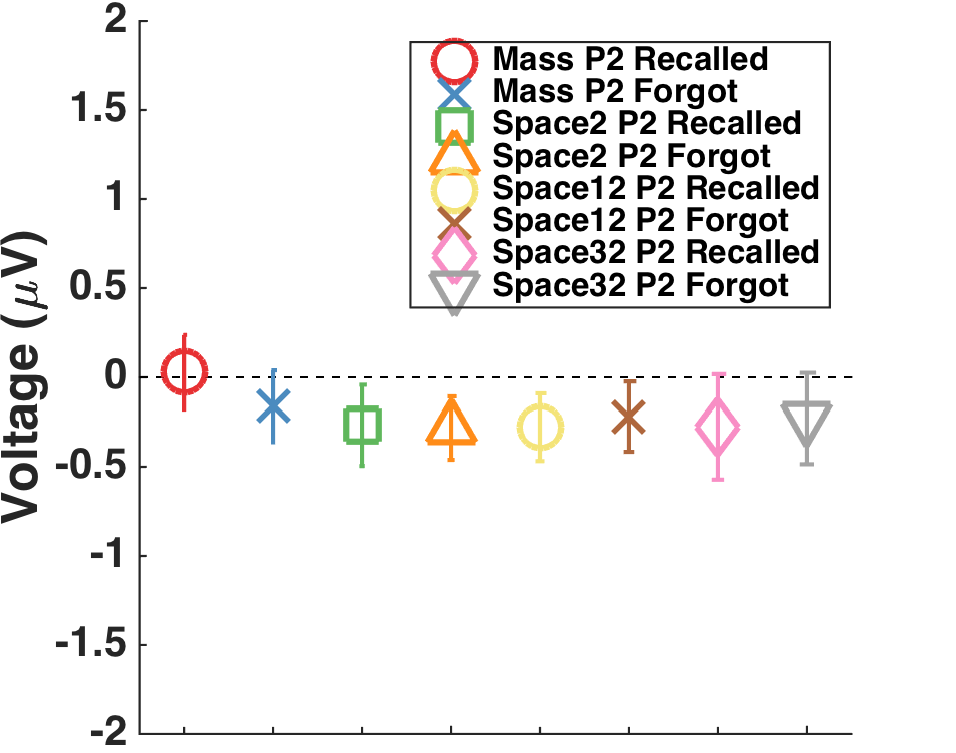
\includegraphics[width=.35\textwidth]{./figs/exp2/tla_avg_ga_word_rc_mass_p2_word_fo_mass_p2_word_rc_spac2_p2_word_fo_spac2_p2_word_rc_spac12_p2_word_fo_spac12_p2_word_rc_spac32_p2_word_fo_spac32_p2_E50_E51_E57_E58_E59_E64_E65_94_194_ylabel}} \\
  \end{tabular}
  \caption{N1 to words at electrode 58 (T5) and neighbors, analyzed window 94--194~ms: (a) Massed ERPs; (b) short spaced ERPs; (c) medium spaced ERPs; (d) long spaced ERPs; (e) analyzed means (error bars are SEM).  The early negative peak is not different across spaced and massed conditions.}
  \label{fig:s2_N1}
  %Figure~\ref{fig:s2_N1}
\end{figure}

If selective attention is modulated by spacing, early ERP components may show effects; this is relevant to deficient processing.  However, there were no significant effects for N1 voltage in the full ANOVA. \cbstart  Because of \textit{a priori} interest based on the results from Experiment~1, we examined the pairwise comparisons in the three-way interaction, which was significant in Experiment~1.  Recalled medium (12) spaced repetitions were marginally more negative ($M=-0.27~\mu$V) than recalled massed repetitions ($M=0.03~\mu$V) [$t(26)=1.99, p=.057$].  The difference compared to massed items was also marginal for recalled short (2) spaced items ($M=-0.26~\mu$V) [$t(26)=2.04, p=.052$] but not so for recalled long (32) spaced items ($M=-0.27~\mu$V) [$t(26)=-1.26, p=0.22$].  Forgotten conditions were all slightly attenuated.  The overall pattern of results is similar to Experiment~1.\cbend

% plot: N400 at Cz + surround
\begin{figure}[hp]
  \centering
  \begin{tabular}{cc}
  %Massed & Spaced-2 \\
  \multicolumn{1}{c}{(a) Massed} & \multicolumn{1}{c}{(b) Spaced-2} \\
  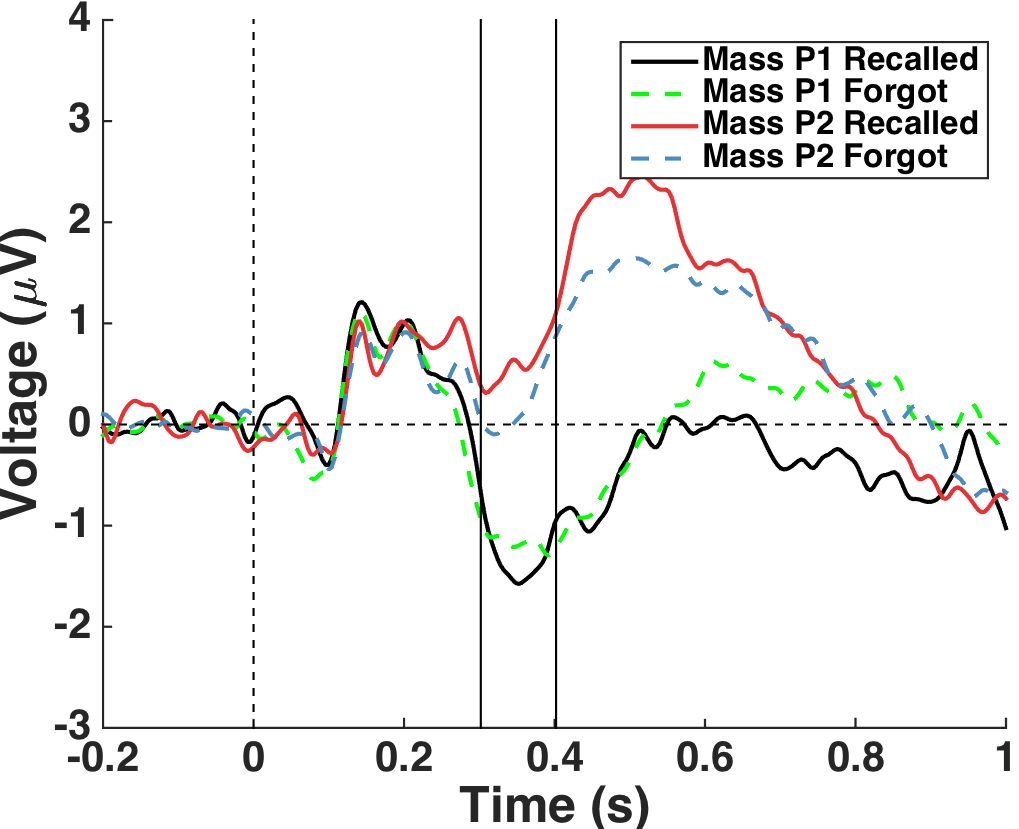
\includegraphics[width=.35\textwidth]{./figs/exp2/tla_single_ga_word_rc_mass_p1_word_fo_mass_p1_word_rc_mass_p2_word_fo_mass_p2_C_-200_1000_legend_xylabel} &
  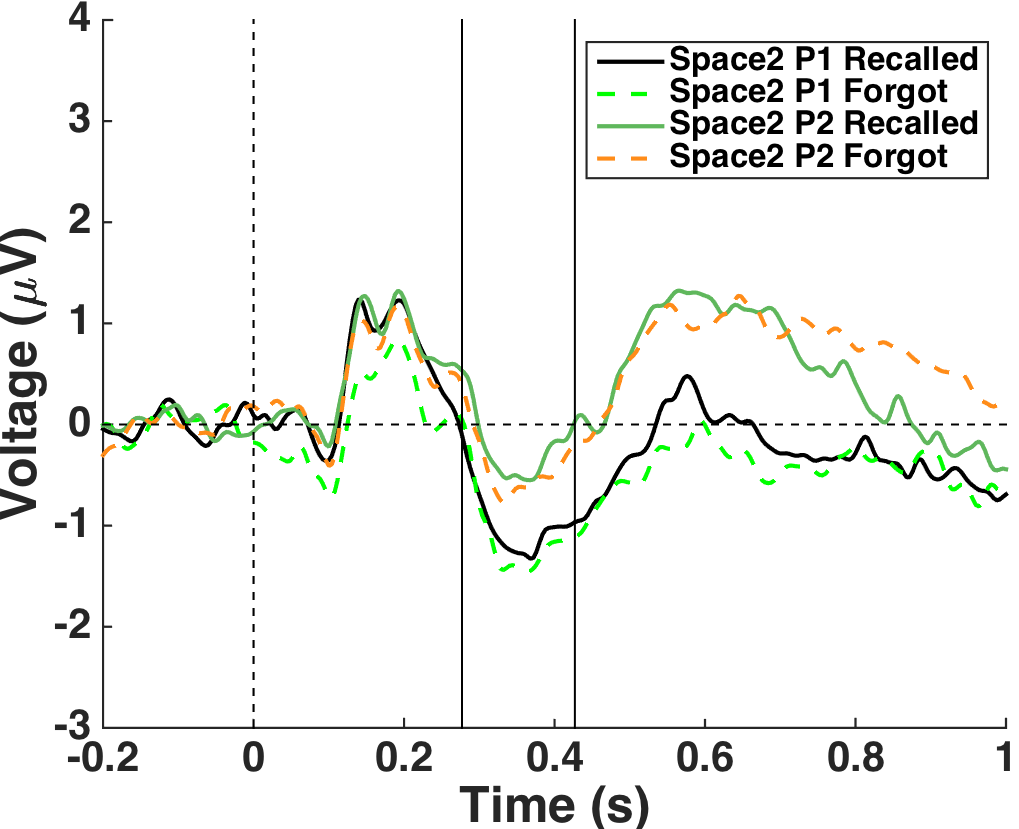
\includegraphics[width=.35\textwidth]{./figs/exp2/tla_single_ga_word_rc_spac2_p1_word_fo_spac2_p1_word_rc_spac2_p2_word_fo_spac2_p2_C_-200_1000_legend_xylabel} \\
  %Spaced-12 & Spaced-32 \\
  \multicolumn{1}{c}{(c) Spaced-12} & \multicolumn{1}{c}{(d) Spaced-32} \\
  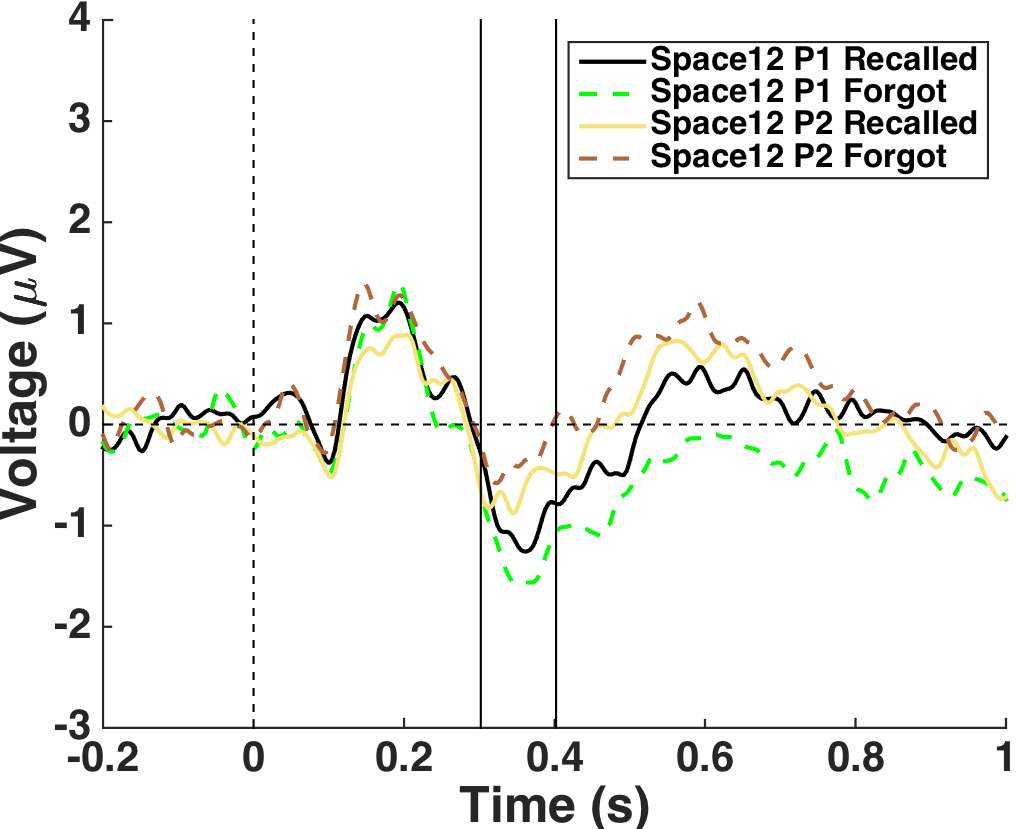
\includegraphics[width=.35\textwidth]{./figs/exp2/tla_single_ga_word_rc_spac12_p1_word_fo_spac12_p1_word_rc_spac12_p2_word_fo_spac12_p2_C_-200_1000_legend_xylabel} &
  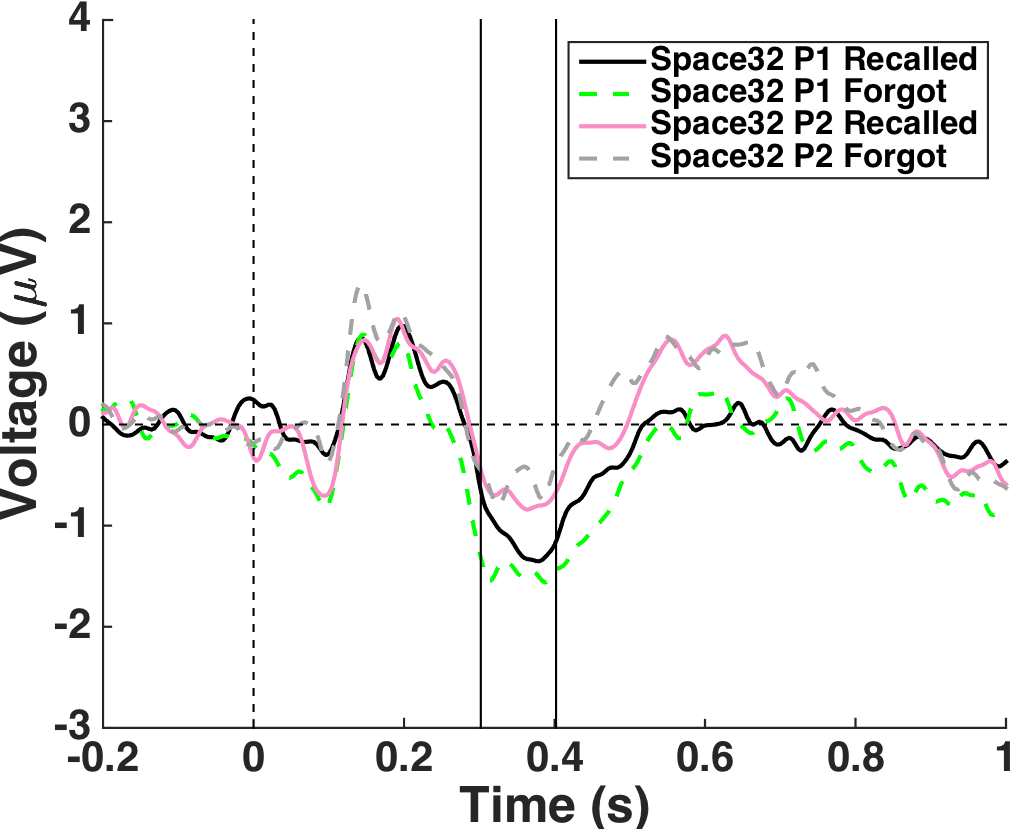
\includegraphics[width=.35\textwidth]{./figs/exp2/tla_single_ga_word_rc_spac32_p1_word_fo_spac32_p1_word_rc_spac32_p2_word_fo_spac32_p2_C_-200_1000_legend_xylabel} \\
  \multicolumn{2}{c}{(e) Means} \\
  \multicolumn{2}{c}{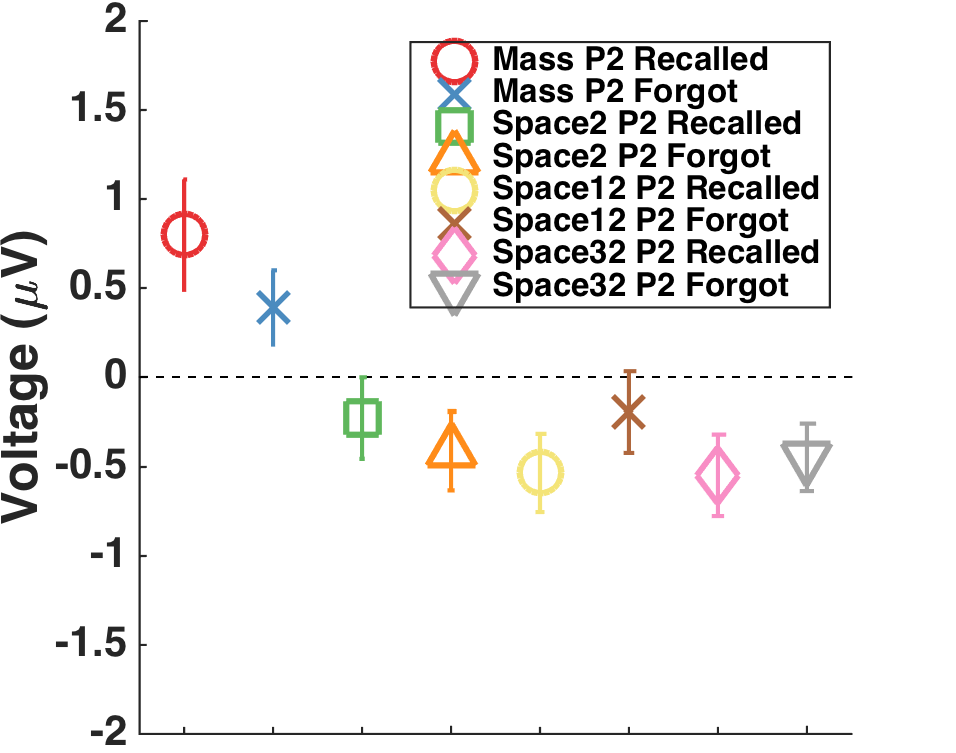
\includegraphics[width=.35\textwidth]{./figs/exp2/tla_avg_ga_word_rc_mass_p2_word_fo_mass_p2_word_rc_spac2_p2_word_fo_spac2_p2_word_rc_spac12_p2_word_fo_spac12_p2_word_rc_spac32_p2_word_fo_spac32_p2_C_277_427_ylabel}} \\
  \end{tabular}
  \caption{N400 to words at electrode Cz and neighbors, analyzed window 227--427~ms: (a) Massed ERPs; (b) short spaced ERPs; (c) medium spaced ERPs; (d) long spaced ERPs; (e) analyzed means (error bars are SEM).  The negative peak at 400~ms is significantly smaller for massed repetitions compared to any spaced repetition condition.}
  \label{fig:s2_N400}
  %Figure~\ref{fig:s2_N400}
\end{figure}


If differences in semantic priming and processing contribute to the spacing effect, the N400 should show effects.
For N400 voltage there was a significant spacing $\times$ presentation interaction [$F(3,78)=8.89, p=6.36e^{-5}$] such that voltage became less negative from first presentations to spaced repetitions to massed repetitions [$p$s~$<.01$].  There were no lag effects (no quantitative differences between spaced conditions).  There were also main effects of spacing (spaced items were more negative than massed [$F(3,78)=11.4, p=2.85e^{-6}$]) and presentation (repetitions were less negative than initial presentations [$F(1,26)=53.2, p=9.5e^{-8}$]).  Finally, there was a three-way interaction [$F(3,78)=2.93, p<.05$].  There were no differences for the initial presentations.  Rather, the effect seems to be driven by recalled medium (12) spaced repetitions showing a negative subsequent memory effect: medium (12) recalled items were more negative than forgotten (recalled: $M=-0.53~\mu$V, forgotten: $M=-0.19~\mu$V) [$t(26)=2.45, p<.05$].  
The two-way interaction, attenuation for massed compared to spaced trials, attenuation for repetitions, and medium (12) SME are the same patterns as seen in Experiment~1.

% This is just a main effect of spacing:
% Recalled trials for short, medium, and long (recalled: $M=-0.54~\mu$V) repetitions were more negative than both massed recalled and forgotten repetitions (recalled: $M=0.8~\mu$V; forgotten: $M=0.39~\mu$V) [$p$s~$<.05$].
% % while remembered massed repetitions showed a marginal positive SME [$t(26)=-1.78, p=.087$].

% There was an effect of latency (spacing x presentation). Mass P2 is faster than all other P2s. I think this might be influenced by the LPC, so I don't think it should be reported.


% plot: LPC at E77 + surround
\begin{figure}[hp]
  \centering
  \begin{tabular}{cc}
  %Massed & Spaced-2 \\
  \multicolumn{1}{c}{(a) Massed} & \multicolumn{1}{c}{(b) Spaced-2} \\
  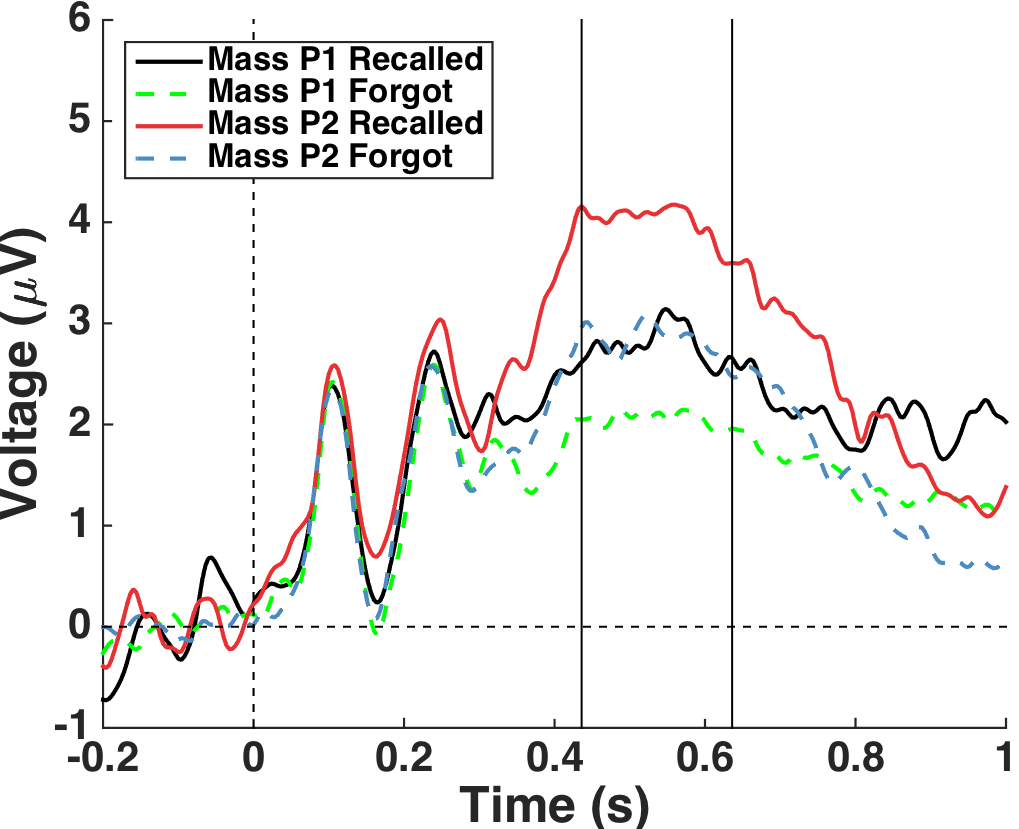
\includegraphics[width=.35\textwidth]{./figs/exp2/tla_single_ga_word_rc_mass_p1_word_fo_mass_p1_word_rc_mass_p2_word_fo_mass_p2_E62_E72_E76_E77_E78_E84_E85_-200_1000_legend_xylabel} &
  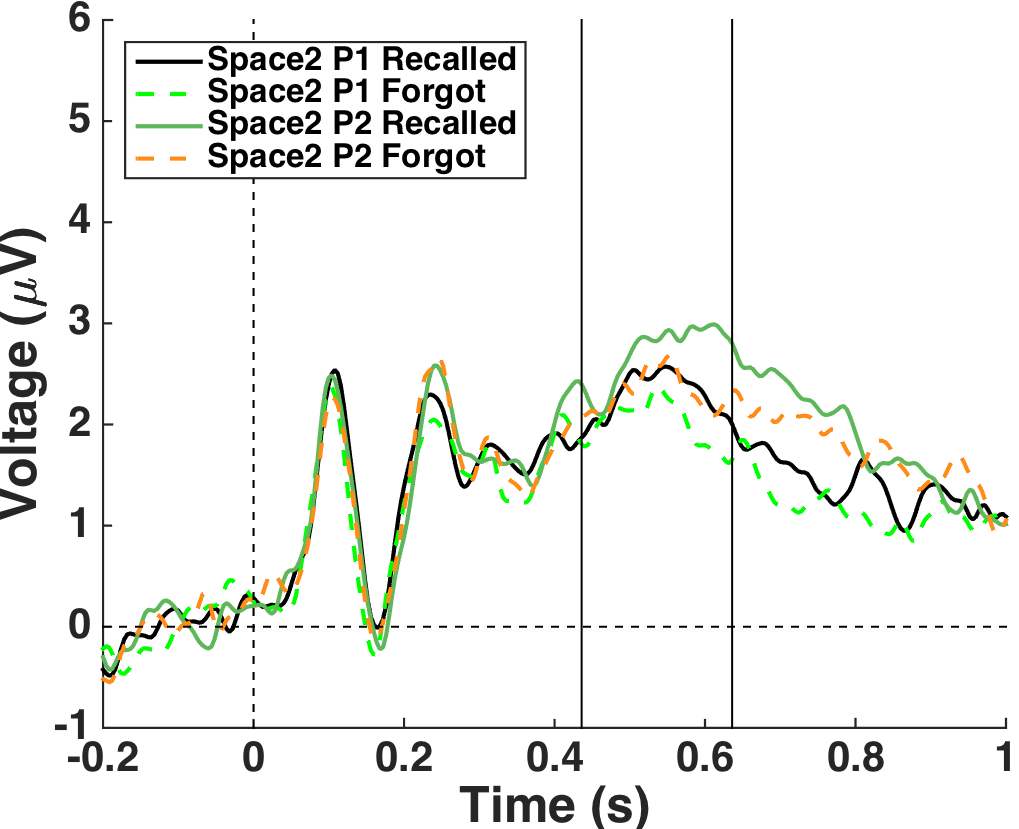
\includegraphics[width=.35\textwidth]{./figs/exp2/tla_single_ga_word_rc_spac2_p1_word_fo_spac2_p1_word_rc_spac2_p2_word_fo_spac2_p2_E62_E72_E76_E77_E78_E84_E85_-200_1000_legend_xylabel} \\
  %Spaced-12 & Spaced-32 \\
  \multicolumn{1}{c}{(c) Spaced-12} & \multicolumn{1}{c}{(d) Spaced-32} \\
  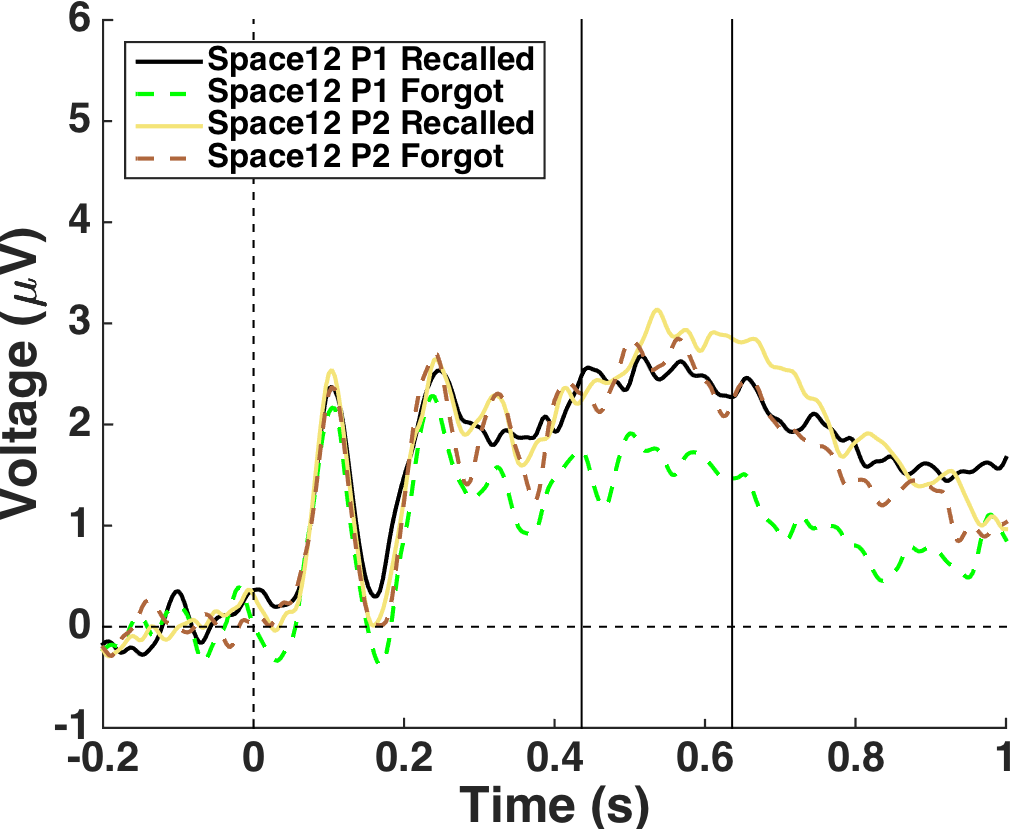
\includegraphics[width=.35\textwidth]{./figs/exp2/tla_single_ga_word_rc_spac12_p1_word_fo_spac12_p1_word_rc_spac12_p2_word_fo_spac12_p2_E62_E72_E76_E77_E78_E84_E85_-200_1000_legend_xylabel} &
  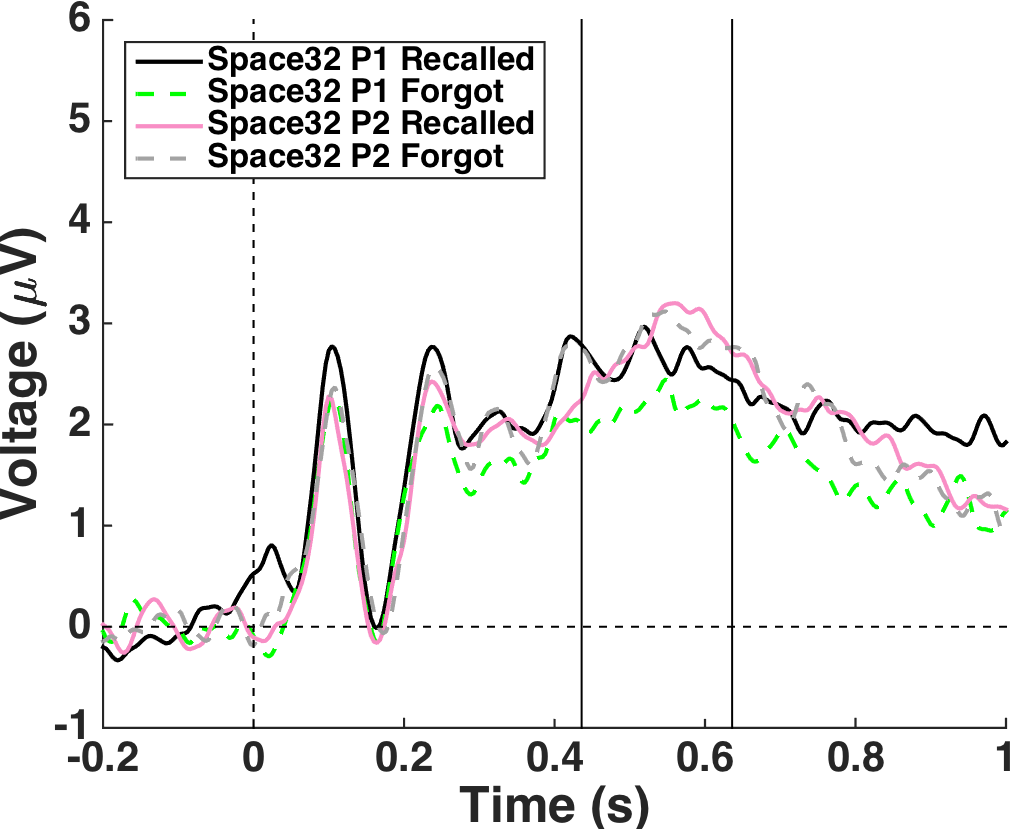
\includegraphics[width=.35\textwidth]{./figs/exp2/tla_single_ga_word_rc_spac32_p1_word_fo_spac32_p1_word_rc_spac32_p2_word_fo_spac32_p2_E62_E72_E76_E77_E78_E84_E85_-200_1000_legend_xylabel} \\
  \multicolumn{2}{c}{(e) Means} \\
  \multicolumn{2}{c}{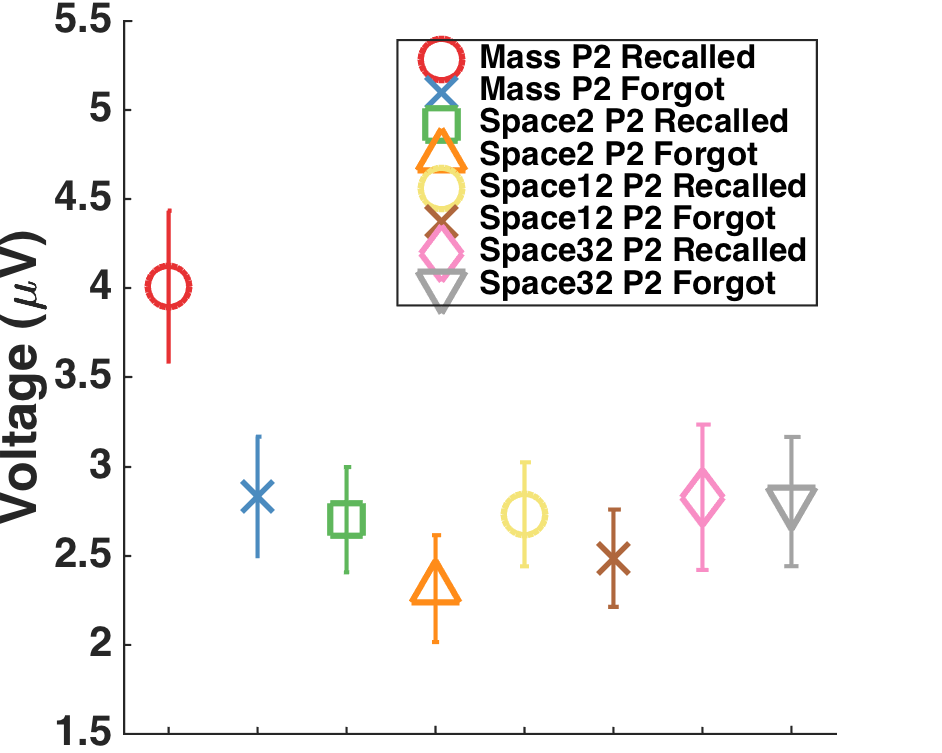
\includegraphics[width=.35\textwidth]{./figs/exp2/tla_avg_ga_word_rc_mass_p2_word_fo_mass_p2_word_rc_spac2_p2_word_fo_spac2_p2_word_rc_spac12_p2_word_fo_spac12_p2_word_rc_spac32_p2_word_fo_spac32_p2_E62_E72_E76_E77_E78_E84_E85_436_636_ylabel}} \\
  \end{tabular}
  \caption{LPC to words at electrode 77 and neighbors, analyzed window 436--636~ms: (a) Massed ERPs; (b) short spaced ERPs; (c) medium spaced ERPs; (d) long spaced ERPs; (e) analyzed means (error bars are SEM).  The positive peak around 600~ms is significantly larger for massed compared to spaced repetitions.}
  \label{fig:s2_LPC}
  %Figure~\ref{fig:s2_LPC}
\end{figure}


The LPC has been linked to the conscious recognition of stimuli in repetition paradigms (particularly those in working memory, as shown in Experiment~1), and may show subsequent memory effects.
For LPC voltage, there were main effects of spacing [$F(3,78)=5.68, p<.005$], presentation [$F(1,26)=31.6, p=6.52e^{-6}$], and memory [$F(1,26)=22.4, p=6.88e^{-5}$].  Massed words ($M=2.92~\mu$V) were more positive than short ($M=2.33~\mu$V) and medium ($M=2.33~\mu$V) spaced words, but only marginally more than long spaced words ($M=2.6~\mu$V) [$t(26)=1.871, p=.073$]; long spaced words were also marginally more positive than short and medium trials [$p$s~$<.1$].  On average, repetitions ($M=2.4~\mu$V) were more positive than initial presentations ($M=2.25~\mu$V), and subsequently recalled words ($M=2.81~\mu$V) were more positive than forgotten ($M=2.28~\mu$V) .

There was no three-way voltage interaction or interaction between spacing and memory in the full ANOVA, but when examining only repetitions using a two-way ANOVA (factors of spacing and memory), there was a significant interaction [$F(3,78)=3.53, p<.05$] showing that massed was the only category with a subsequent memory effect; the actual voltage difference between recalled and forgotten words decreased with lag.
% why would SME decrease with lag? less info retrieved at longer lags.

For LPC latency effects, which illuminate how quickly information is consciously accessed, there was the same spacing $\times$ presentation interaction [$F(3,78)=2.86, p<.05$] as in Experiment~1: medium (544~ms) and long (550~ms) spaced repetitions peaked later than massed repetitions (529~ms) [$p$s~$<.05$]; this pattern was marginal for short spaced repetitions (544~ms) [$t(26)=1.9456, p=.063$].  Spaced repetitions also peaked later than their respective initial presentations (long: 529~ms [$t(26)=3.98, p<.0005$], medium: 532~ms [$t(26)=1.96, p=0.061$] marginal).

\subsection{ERP discussion}

Under deficient processing we expected the N1 for repetitions to show a lag effect (become more negative as lag increases) because increased early attentional processing should lead to better subsequent memory, for which we have shown a clear behavioral lag effect.  For example, a repetition at lag 2 would have a voltage in between a massed item and a repetition at lag 12.  However, for N1 voltage there were no significant effects, though examining pairwise comparisons of the three-way interaction revealed qualitatively similar patterns to Experiment~1:  spaced items in general seem to get more attentional processing than massed items.

Keeping in mind that the overall pattern from Experiment~1 persisted, the lack of significant N1 effects leads to the idea that attention is not the critical factor for why the spacing effect occurs, at least when defining attention as an early involuntary mechanism indexed by the N1.  We cannot make any strong claims in the face of null results, but overall this is less evidence to support deficient processing.

There are a few possibilities to consider for the attenuated N1 effect.
Perhaps an experiment difference such as removing the exposure phase made a difference for the N1 in that having an existing representation of a stimulus before needing to learn stimulus pairings could change attentional mechanisms.

Another possibility is that spaced repetitions were relatively more likely to occur in the second experiment (occurred approximately 75\% of the time) compared to Experiment~1 (occurred approximately 50\% of the time).  Perhaps this made spaced repetitions less attention grabbing.  We could not find any discussion in the literature relating N1 amplitude to relative stimulus frequency.

% \hl{(Perhaps the N1 effects in Experiment~2 went away because spaced repetitions were relatively more likely to occur than in Experiment~1.  Therefore, spaced items were more common and less attention grabbing in Experiment~2.  Have stimulus probability effects been documented for the N1?)}

A third question regarding the lack of N1 effects is how short term the repetition effects are.  \citeA{HensEtal2004} investigated ERP effects for repetitions of pictures of objects at different lags and saw a repetition effect for a similarly timed ERP component (labeled N170, associated with processing faces) after an unfilled 4-second delay (amplitude decreased for repetitions), but not when the four seconds was occupied by another stimulus or at a much longer lag (96 seconds).  Thus, deficient processing of a repetition may be eliminated at a relatively short delay if it is filled with other stimuli.  Regardless of these differences, based on the results from Experiment~1 we expected an N1 attenuation for massed compared to spaced repetitions, and we still saw strong behavioral spacing and lag effects in Experiment~2, so there seem to be other mechanisms involved in these effects.


We expected the N400 to show lag effects, considering its tie to semantic processing: the component would get more negative as lag increases because more semantic activation is needed during retrieval for longer lags.  The N400 showed similar results to Experiment~1, but there were no lag effects across spaced conditions, only a difference between massed and spaced items in the expected direction: massed items were strongly attenuated compared to spaced.  The voltage averages (Figure~\ref{fig:s2_N400}e) show an overall pattern of being more negative for remembered items at longer lags.  The only significant effect of memory was for recalled medium (12) spaced repetitions, which aligns with Experiment~1, though there is no reason to think this particular spacing lag is important.

Based on the N400, it seems that a similar amount of semantic processing is engaged when there have been at least two intervening stimulus pairs between repetitions.
These results imply that spaced repetitions (regardless of lag) receive more semantic processing, or conversely that semantic processing disengages more for massed repetitions.  This still supports the \citeA{Chal1993} semantic activation hypothesis (less semantic activation for items in working memory), but only one that posits deficient processing for immediate repetitions, and thus cannot explain the behavioral lag effect.
Therefore, deficient processing provides only a partial explanation.


% This follows the results of Experiment~1.
Finally, we expected working memory effects (LPC) to be graded across lags.  Theoretically, this could occur for two reasons, in opposite directions.  First, in terms of memory retrieval (posited under study-phase retrieval), we might see subsequent memory effects for spaced items.  More retrieval would be needed as lag increases; it should also be more difficult, as described in the models of \citeNP{PavlAnde2005} and \citeNP{MozeEtal2009}, but also more beneficial to long-term memory if it is successful.  This would posit larger LPC effects as lag increases.
Second, the gradation might go in the other direction: effects related to indexing working memory should be stronger for massed items and decrease with lag.  This larger difference of subsequent memory for massed items is what we see: massed repetitions were more positive and peaked earlier than spaced repetitions, and showed an SME.
%Though there were no significant SMEs for spaced items, the pattern of voltage difference decreasing with lag aligns with the idea that less information is retrieved at longer lags.

Also supporting the idea of the LPC indexing conscious access to these representations are the latency effects: their later peaks show that it takes longer to access medium and long spaced representations compared to the massed and short spaced conditions.
As in Experiment~1, it seems that the LPC indexes the information that is in working memory, and again, the result does not seem to directly support any of the theories unless the match to working memory for massed items is an indicator of deficient processing.

% Behavioral performance was higher for spaced items, spaced items were obviously not forgotten even though they did not show an LPC memory effect, so this effect does not seen to be indexing recollection.  This makes sense when comparing its topography (Experiment~1, Figure~\ref{fig:LPC}, page~\pageref{fig:LPC}) to the parietal old/new effect in the literature associated with recollection, which is typically more left parietal.

% The LPC showed that information is being retrieved during repetitions (higher voltage), particularly for primed and/or still active massed items, as well as for subsequently recalled words overall.
% The two-way ANOVA for repetitions indicates that information is more easily retrieved from memory at shorter lags.  Or, perhaps it shows that higher voltage matters more at shorter lags for subsequent memory performance.  Since performance was best for the long (32) spaced repetitions, under the study-phase retrieval hypothesis we would expect a sign of retrieval.  However, we did not find this.

Though we have found some support for deficient processing, specifically in relation to massed items, the mechanisms involved in this hypothesis seem to have little bearing on the spaced conditions and therefore cannot capture the lag effect.  Thus, we still have not found a defining neural signature for why performance increases with lag.

\subsection{Time--frequency results}

As in Experiment~1, we analyzed images in addition to words for time--frequency data.
Three-way ANOVAs with factors of spacing (spaced and massed), subsequent memory (recalled and forgotten), and time (0--500~ms and 500--1000~ms) were performed for word and image repetitions on power in the theta, lower alpha, upper alpha, and lower beta bands (eight ANOVAs).


% plot: word and image theta
\begin{figure}[H]
  \centering
  \begin{tabular}{cccc}
  & Theta power & Theta power & Means \\
  & \multicolumn{1}{l}{(a)} & \multicolumn{1}{l}{(b)} & \multicolumn{1}{l}{(c)} \\
  \raisebox{1.8cm}{\rotatebox{90}{Word}} & 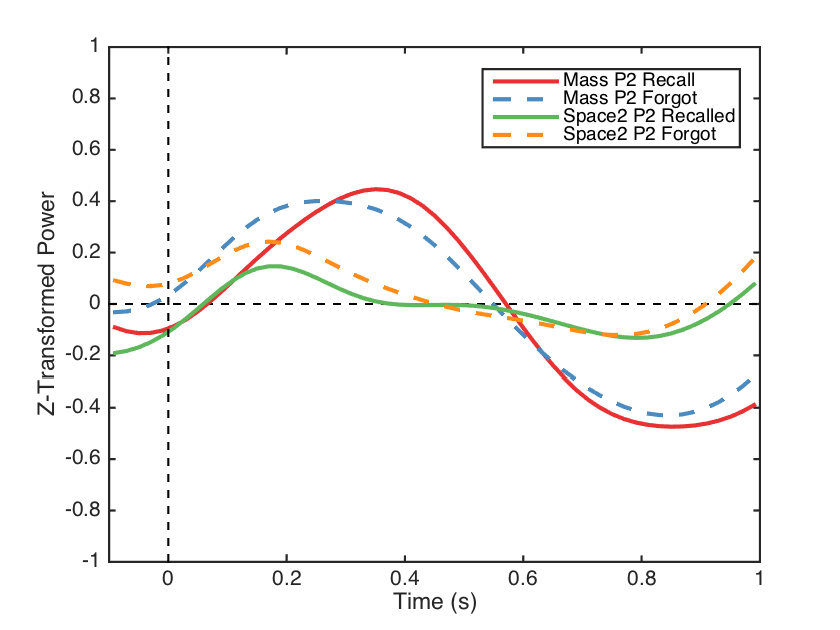
\includegraphics[width=.30\textwidth]{./figs/exp2/tfr_line/tfr_line_ga_word_rc_mass_p2_word_fo_mass_p2_word_rc_spac2_p2_word_fo_spac2_p2_4_8_-100_1000_73ROIs_legend} &
  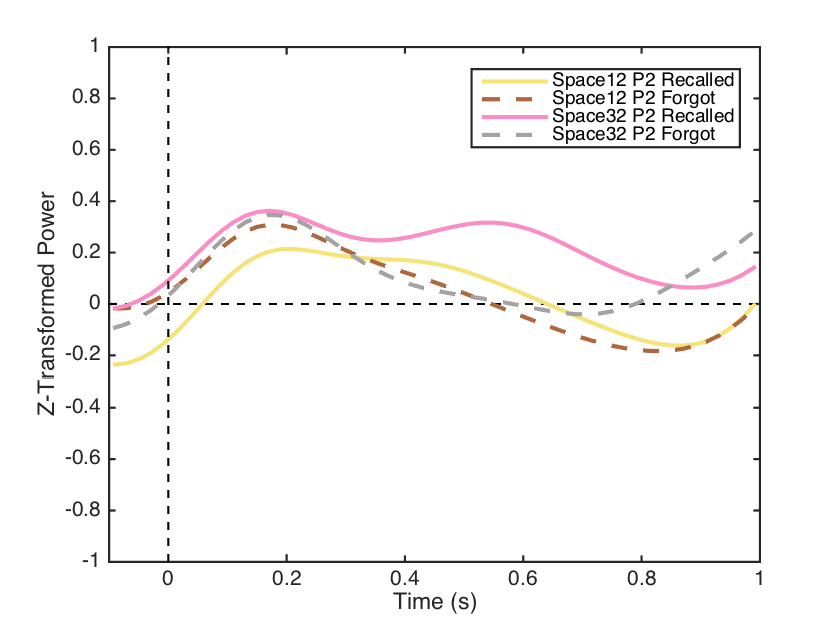
\includegraphics[width=.30\textwidth]{./figs/exp2/tfr_line/tfr_line_ga_word_rc_spac12_p2_word_fo_spac12_p2_word_rc_spac32_p2_word_fo_spac32_p2_4_8_-100_1000_73ROIs_legend} &
  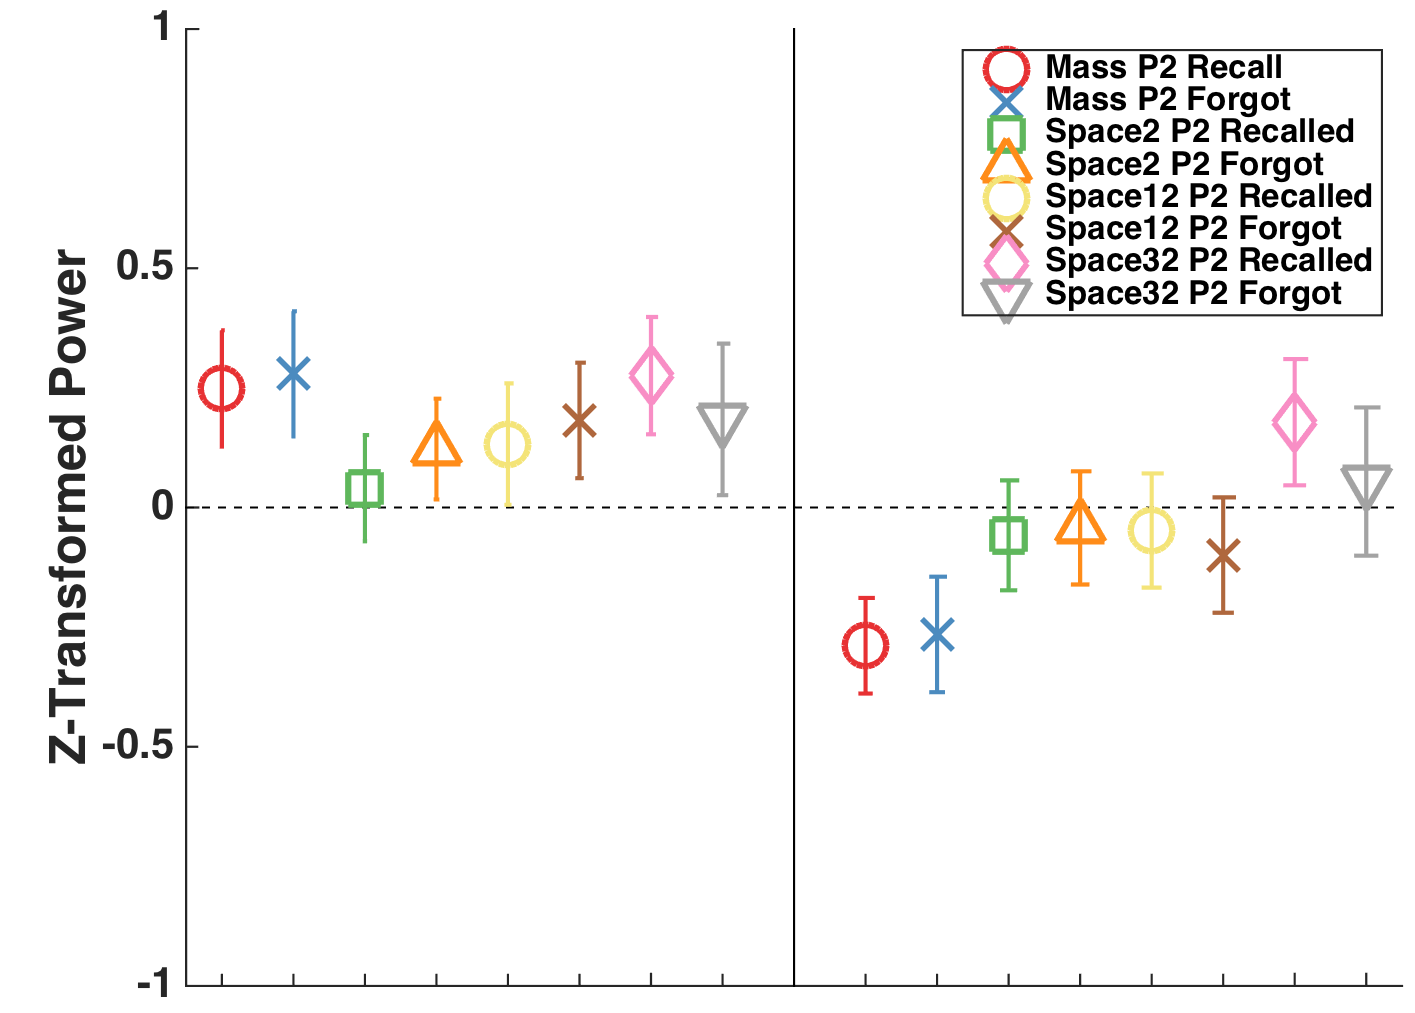
\includegraphics[width=.30\textwidth]{./figs/exp2/tfr_avg/tfr_avg_ga_word_rc_mass_p2_word_fo_mass_p2_word_rc_spac2_p2_word_fo_spac2_p2_word_rc_spac12_p2_word_fo_spac12_p2_word_rc_spac32_p2_word_fo_spac32_p2_4_8_0_500_500_1000_73ROI_ylabel} \\
  & \multicolumn{1}{l}{(d)} & \multicolumn{1}{l}{(e)} & \multicolumn{1}{l}{(f)} \\
  \raisebox{1.8cm}{\rotatebox{90}{Image}} & 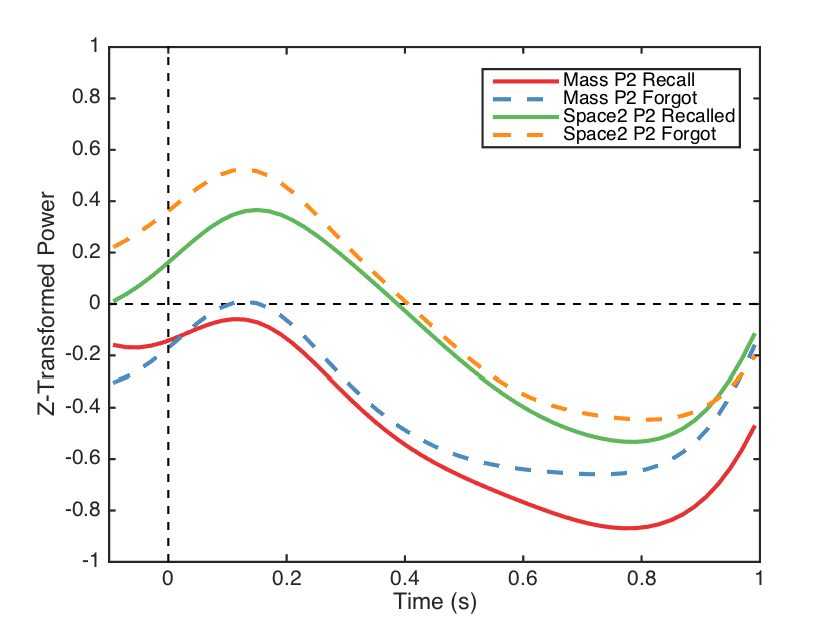
\includegraphics[width=.30\textwidth]{./figs/exp2/tfr_line/tfr_line_ga_img_rc_mass_p2_img_fo_mass_p2_img_rc_spac2_p2_img_fo_spac2_p2_4_8_-100_1000_90ROIs_legend} &
  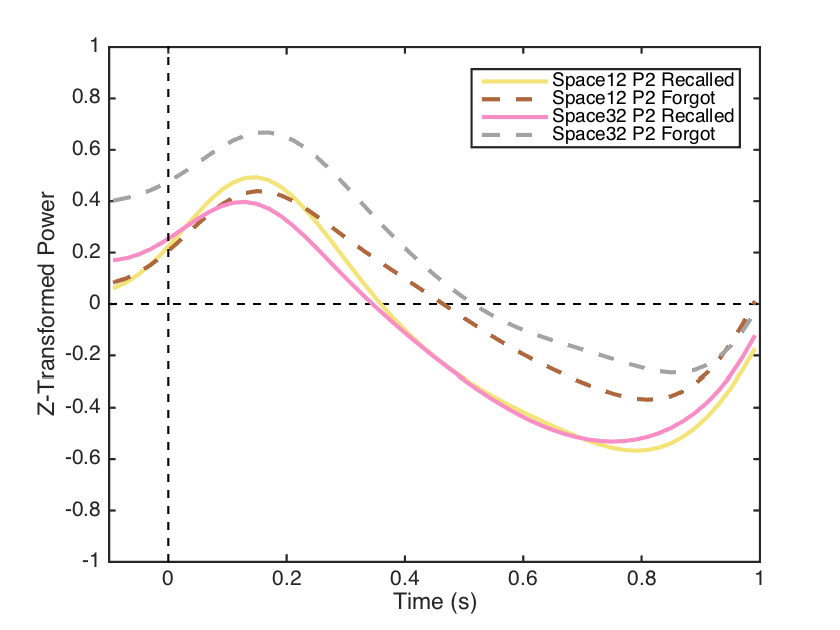
\includegraphics[width=.30\textwidth]{./figs/exp2/tfr_line/tfr_line_ga_img_rc_spac12_p2_img_fo_spac12_p2_img_rc_spac32_p2_img_fo_spac32_p2_4_8_-100_1000_90ROIs_legend} &
  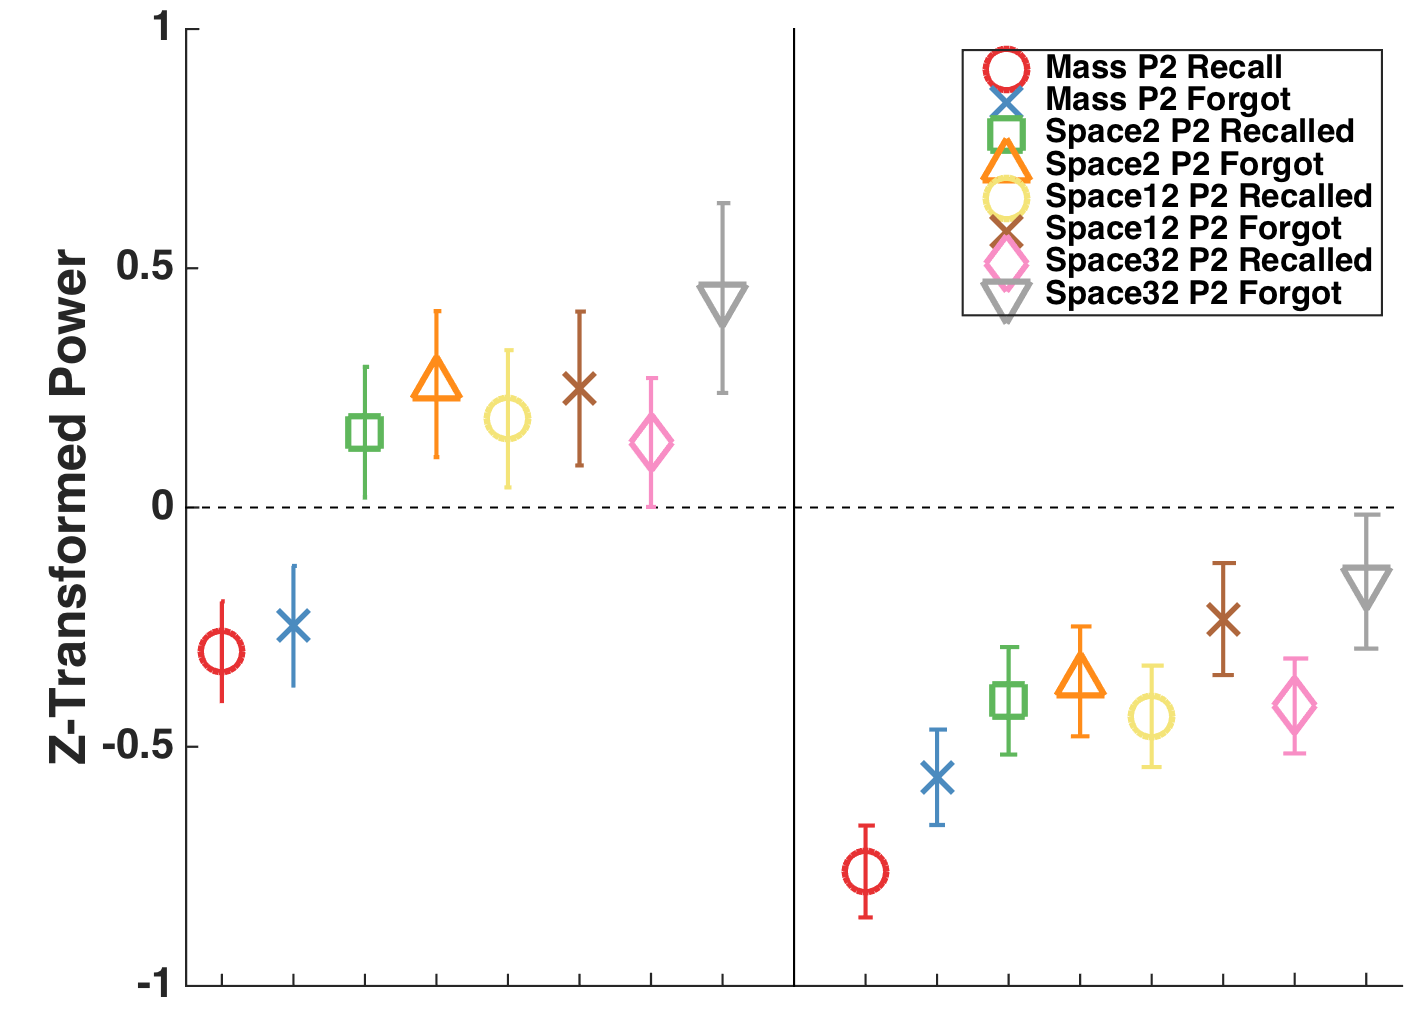
\includegraphics[width=.30\textwidth]{./figs/exp2/tfr_avg/tfr_avg_ga_img_rc_mass_p2_img_fo_mass_p2_img_rc_spac2_p2_img_fo_spac2_p2_img_rc_spac12_p2_img_fo_spac12_p2_img_rc_spac32_p2_img_fo_spac32_p2_4_8_0_500_500_1000_90ROI_ylabel} \\
  \end{tabular}
  \caption{Theta power to words and images.  (a), (b), (d), and (e) Grand averages; (c) and (f) mean values for the two time windows (error bars are SEM).}
  \label{fig:s2_word_img_theta}
  %Figure~\ref{fig:s2_word_img_theta}
\end{figure}

% words
\textit{Word, theta}: Across 73 electrodes (Figure~\ref{fig:s2_word_img_theta}, top), there was a spacing $\times$ time interaction [$F(3,78)=16, p=5.33e^{-8}$] such that all conditions decreased across time [$p$s~$<.05$] except long (32) spaced words.  Contributing to this were main effects of spacing [$F(3,78)=4.0, p<.05$] and time [$F(1,26)=33, p=4.81e^{-6}$].  Long (32) spaced word repetitions showed more theta power than all other conditions [$p$s~$<.05$], and there was a decrease in power across time.
There was no three-way interaction, but pairwise comparisons for recalled words between massed and spaced conditions in the later time window showed that long (32) spaced words had significantly higher theta power than all other conditions.

\textit{Image, theta}: Across 90 electrodes (Figure~\ref{fig:s2_word_img_theta}, bottom), there were main effects of spacing [$F(3,78)=27.2, p=1.17e^{-10}$], memory [$F(1,26)=8.76, p<.01$], and time [$F(1,26)=91.1, p=5.57e^{-10}$].  Massed items desynchronized more overall than the other conditions, subsequently recalled items desynchronized more than forgotten ones, and power decreased across time.  A spacing $\times$ time interaction [$F(3,78)=5.14, p<.01$] showed that the decrease in power across time for massed items was less than short (2) and medium (12) spaced repetitions.

% plot: word and image lower alpha
\begin{figure}[H]
  \centering
  \begin{tabular}{cccc}
  & Lower alpha power & Lower alpha power & Means \\
  & \multicolumn{1}{l}{(a)} & \multicolumn{1}{l}{(b)} & \multicolumn{1}{l}{(c)} \\
  \raisebox{1.8cm}{\rotatebox{90}{Word}} & 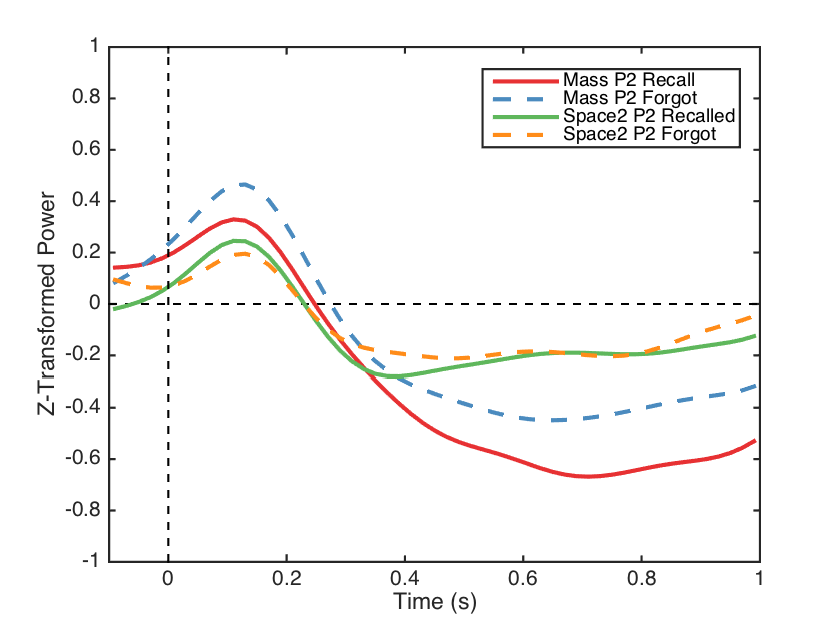
\includegraphics[width=.30\textwidth]{./figs/exp2/tfr_line/tfr_line_ga_word_rc_mass_p2_word_fo_mass_p2_word_rc_spac2_p2_word_fo_spac2_p2_8_10_-100_1000_49ROIs_legend} &
  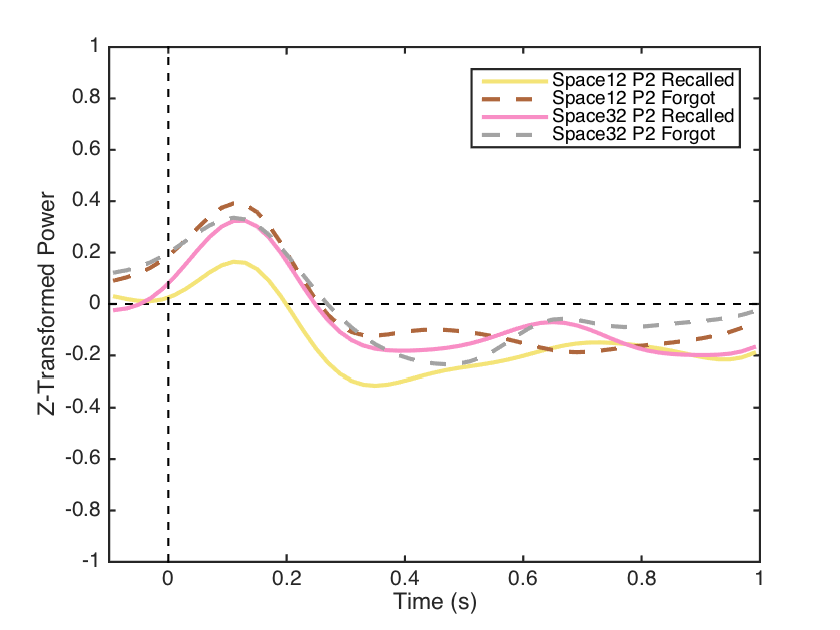
\includegraphics[width=.30\textwidth]{./figs/exp2/tfr_line/tfr_line_ga_word_rc_spac12_p2_word_fo_spac12_p2_word_rc_spac32_p2_word_fo_spac32_p2_8_10_-100_1000_49ROIs_legend} &
  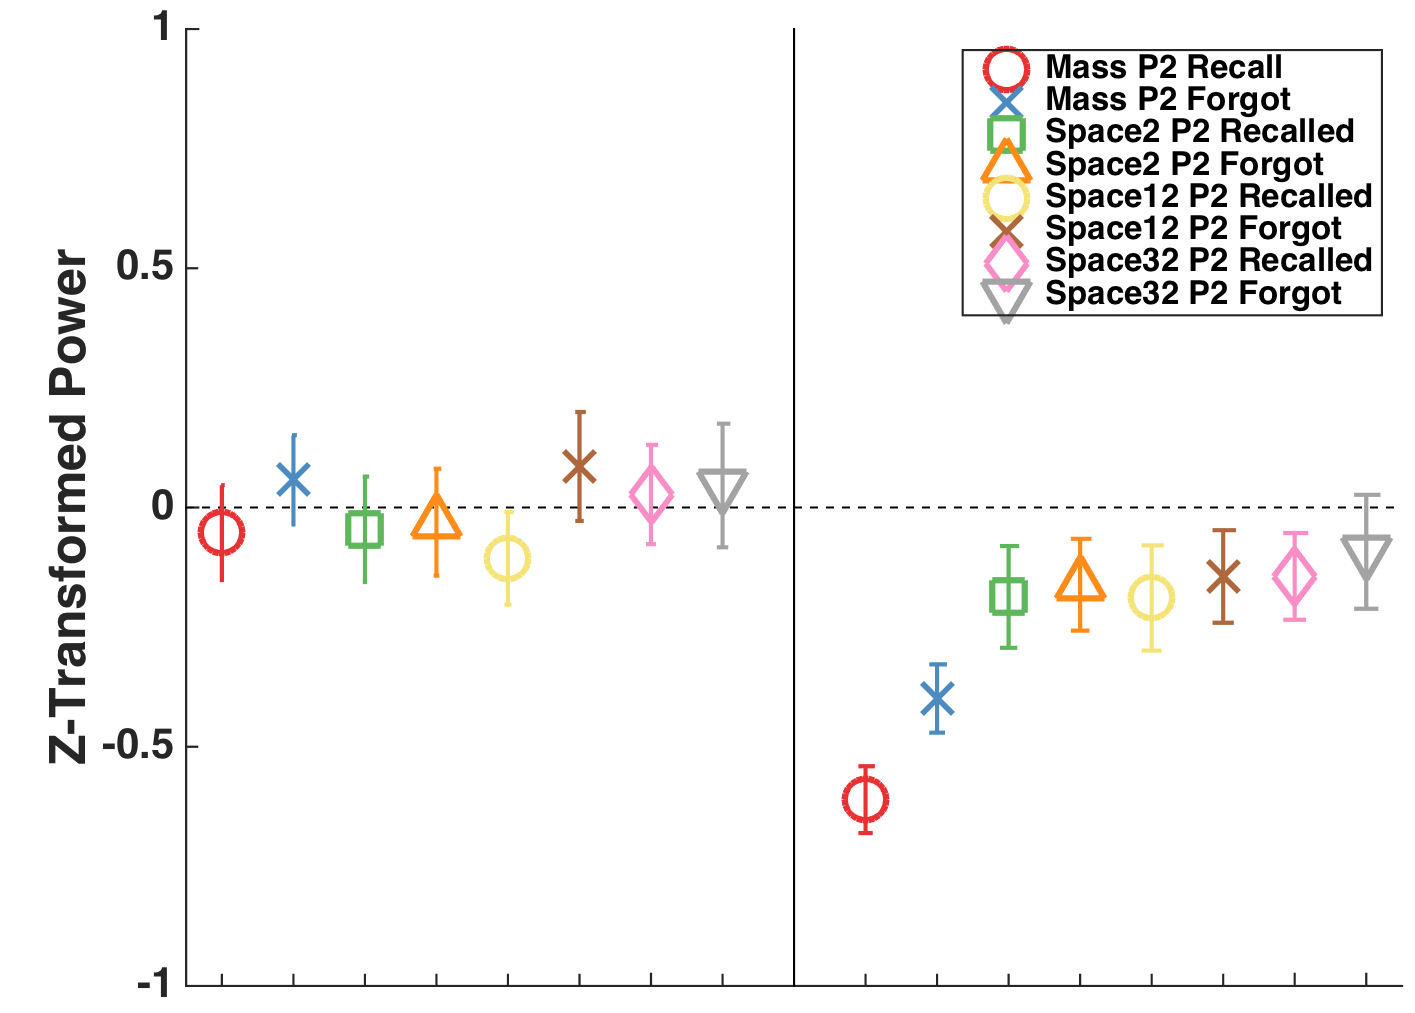
\includegraphics[width=.30\textwidth]{./figs/exp2/tfr_avg/tfr_avg_ga_word_rc_mass_p2_word_fo_mass_p2_word_rc_spac2_p2_word_fo_spac2_p2_word_rc_spac12_p2_word_fo_spac12_p2_word_rc_spac32_p2_word_fo_spac32_p2_8_10_0_500_500_1000_49ROI_ylabel} \\
  & \multicolumn{1}{l}{(d)} & \multicolumn{1}{l}{(e)} & \multicolumn{1}{l}{(f)} \\
  \raisebox{1.8cm}{\rotatebox{90}{Image}} & 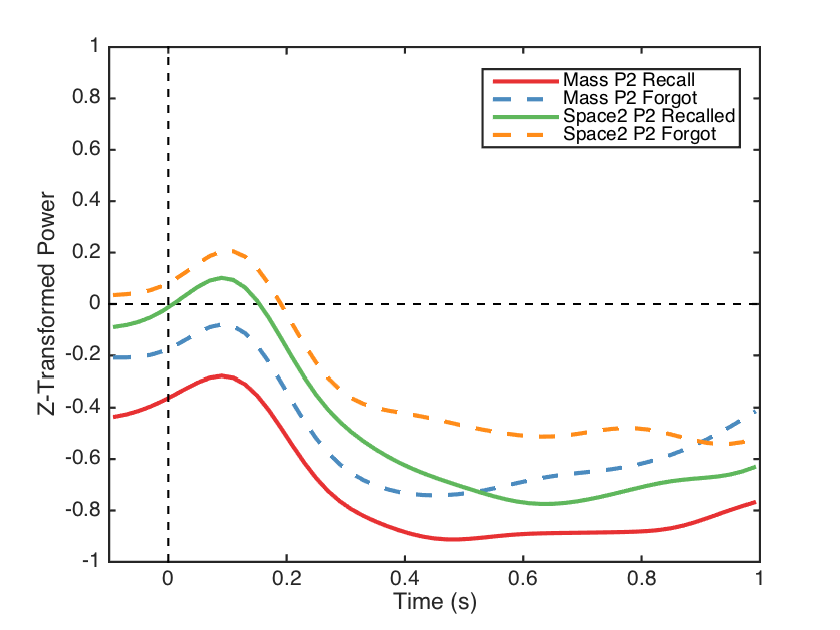
\includegraphics[width=.30\textwidth]{./figs/exp2/tfr_line/tfr_line_ga_img_rc_mass_p2_img_fo_mass_p2_img_rc_spac2_p2_img_fo_spac2_p2_8_10_-100_1000_94ROIs_legend} &
  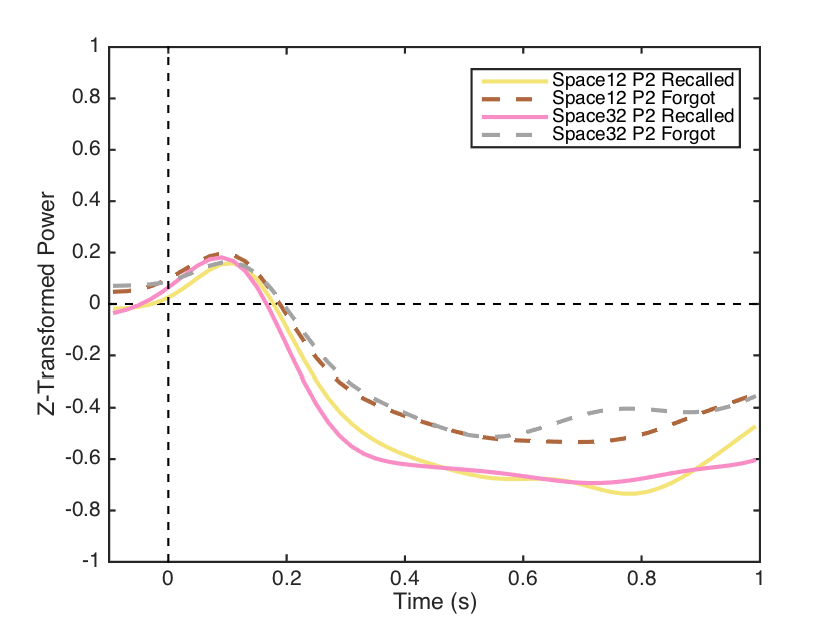
\includegraphics[width=.30\textwidth]{./figs/exp2/tfr_line/tfr_line_ga_img_rc_spac12_p2_img_fo_spac12_p2_img_rc_spac32_p2_img_fo_spac32_p2_8_10_-100_1000_94ROIs_legend} &
  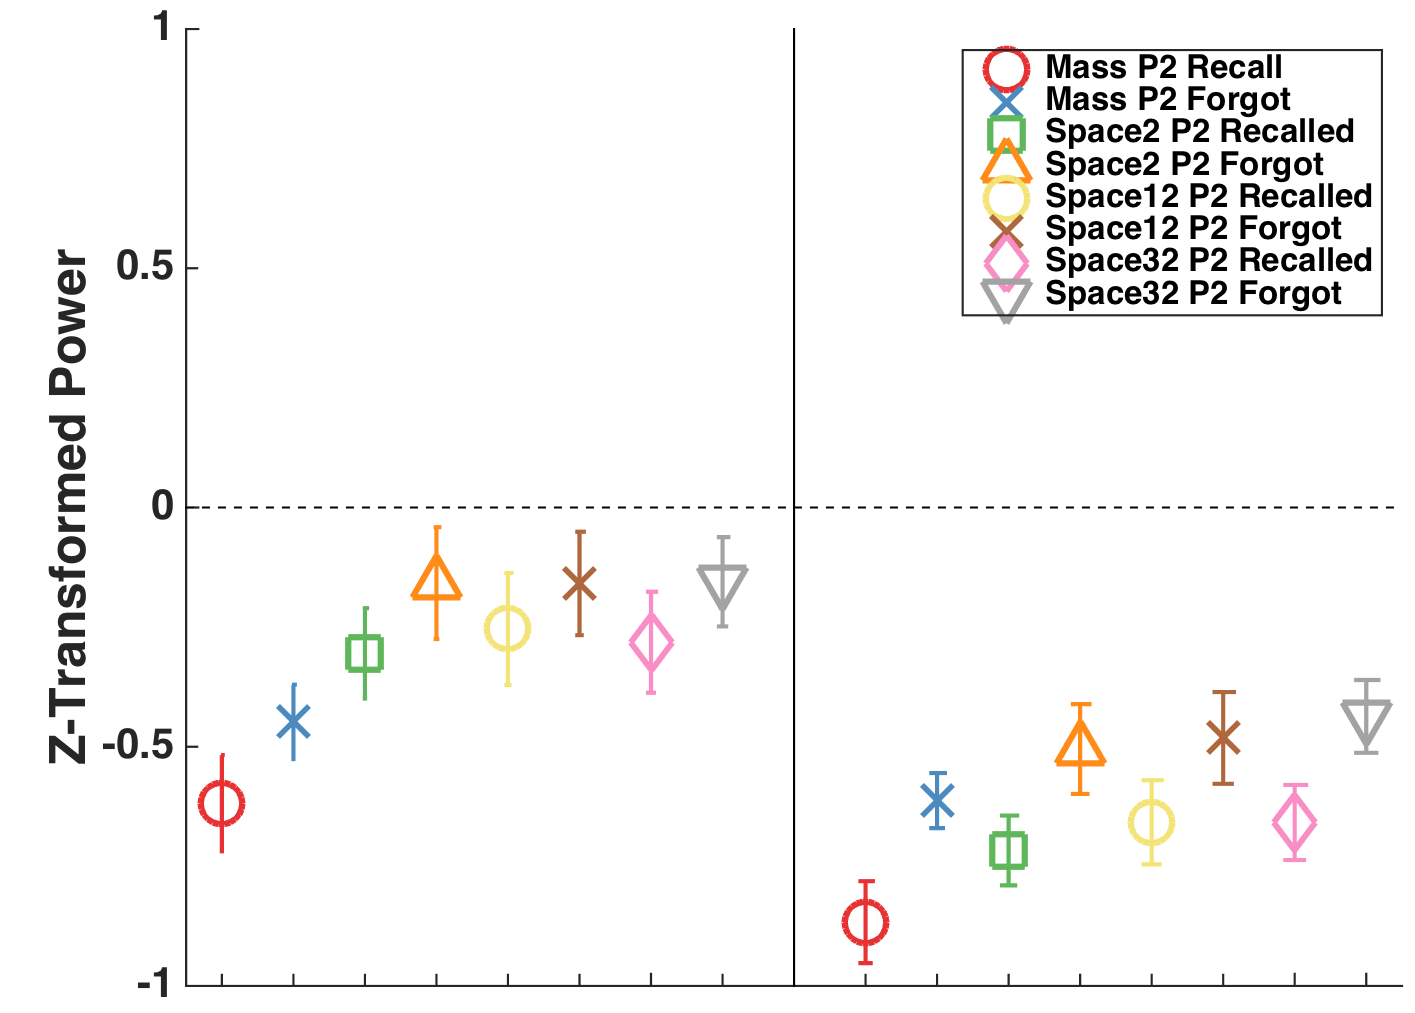
\includegraphics[width=.30\textwidth]{./figs/exp2/tfr_avg/tfr_avg_ga_img_rc_mass_p2_img_fo_mass_p2_img_rc_spac2_p2_img_fo_spac2_p2_img_rc_spac12_p2_img_fo_spac12_p2_img_rc_spac32_p2_img_fo_spac32_p2_8_10_0_500_500_1000_94ROI_ylabel} \\
  \end{tabular}
  \caption{Lower alpha power to words and images.  (a), (b), (d), and (e) Grand averages; (c) and (f) mean values for the two time windows (error bars are SEM).}
  \label{fig:s2_word_img_alpha_low}
  %Figure~\ref{fig:s2_word_img_alpha_low}
\end{figure}


\textit{Word, lower alpha}: Across 49 electrodes (Figure~\ref{fig:s2_word_img_alpha_low}, top), we saw the same spacing $\times$ time interaction [$F(3,78)=15.1, p=2.15e^{-7}$] as in Experiment~1.  Lower alpha desynchronized more (power was more negative) across time windows for massed compared to spaced words.  There were also significant main effects of spacing [$F(3,78)=9.78, p=2.22e^{-5}$], memory [$F(1,26)=5.89, p<.05$], and time [$F(1,26)=9.71, p<.005$].  Massed word repetitions showed more lower alpha desynchronization than the other conditions, there was more desynchronization for recalled images, and there was more desynchronization in the second time window; these effects were the same as in Experiment~1 and seem to be driven by massed recalled items.


\textit{Image, lower alpha}: Across 94 electrodes (Figure~\ref{fig:s2_word_img_alpha_low}, bottom), lower alpha for images showed the same pattern of effects as for words; these are also the same effects as from Experiment~1.  There was a spacing $\times$ time interaction [$F(3,78)=6.23, p<.005$] that showed a larger decrease for spaced items across time compared to massed.  There were main effects of spacing [$F(3,78)=14.3, p=2.65e^{-7}$] (massed desynchronized more than spaced), memory [$F(1,26)=24.7, p=3.67e^{-5}$] (remembered desynchronized more than forgotten), and time [$F(1,26)=33.6, p=4.19e^{-6}$] (desynchronization decreased over time).  Additionally,  there was a memory $\times$ time interaction [$F(1,26)=5.37, p<.05$]; SMEs were stronger in the later time window.
% aka: recalled items desynchronized more across time than forgotten ones.


% plot: word and image upper alpha
\begin{figure}[H]
  \centering
  \begin{tabular}{cccc}
  & Upper alpha power & Upper alpha power & Means \\
  & \multicolumn{1}{l}{(a)} & \multicolumn{1}{l}{(b)} & \multicolumn{1}{l}{(c)} \\
  \raisebox{1.8cm}{\rotatebox{90}{Word}} & 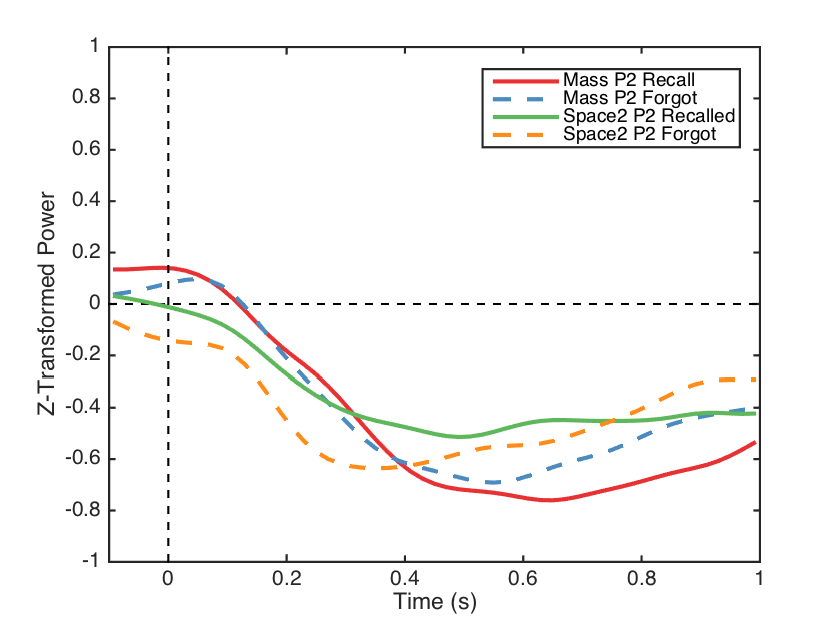
\includegraphics[width=.30\textwidth]{./figs/exp2/tfr_line/tfr_line_ga_word_rc_mass_p2_word_fo_mass_p2_word_rc_spac2_p2_word_fo_spac2_p2_11_12_-100_1000_46ROIs_legend} &
  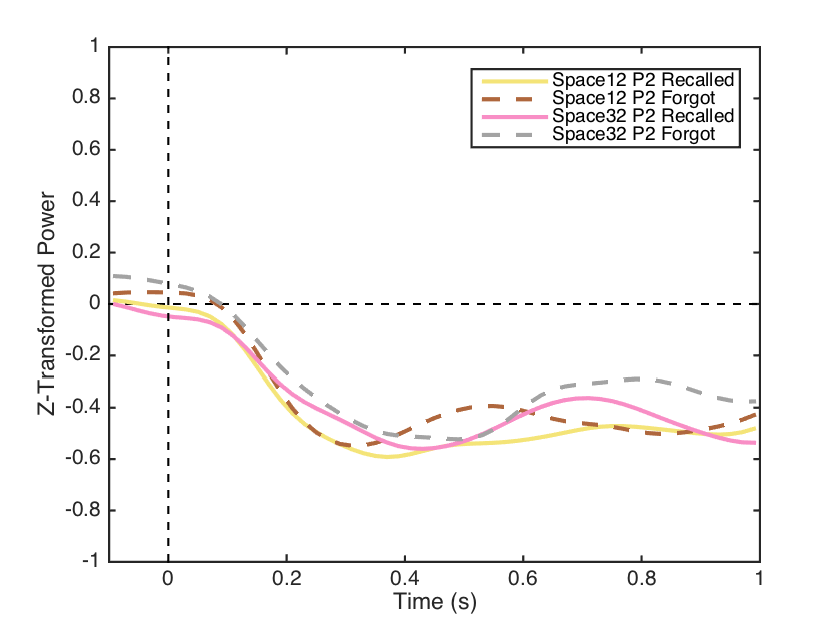
\includegraphics[width=.30\textwidth]{./figs/exp2/tfr_line/tfr_line_ga_word_rc_spac12_p2_word_fo_spac12_p2_word_rc_spac32_p2_word_fo_spac32_p2_11_12_-100_1000_46ROIs_legend} &
  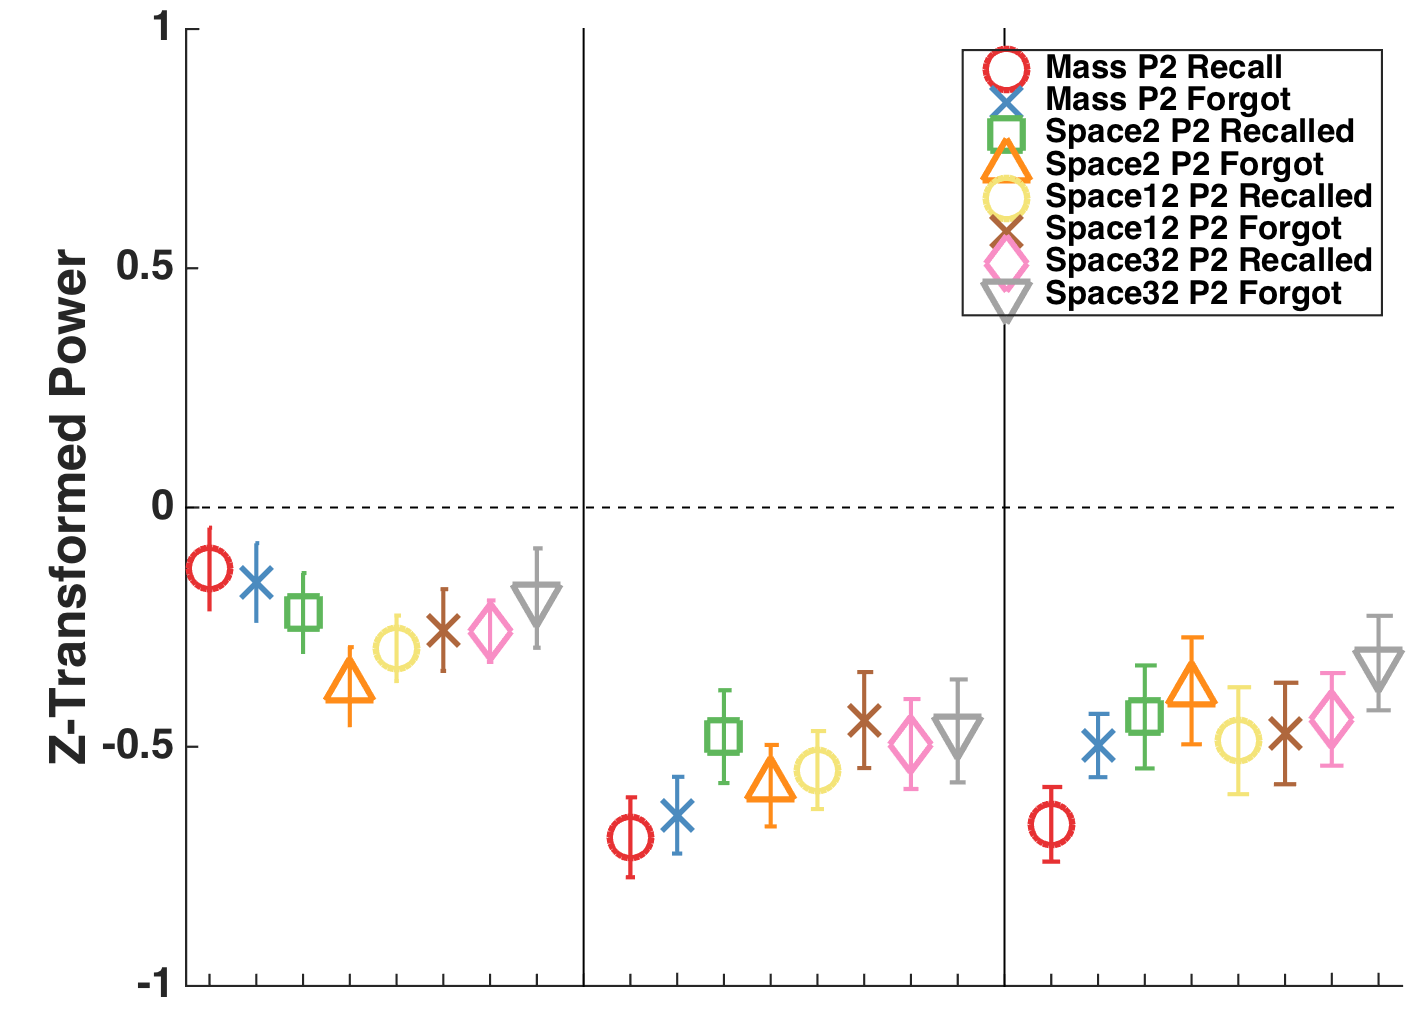
\includegraphics[width=.30\textwidth]{./figs/exp2/tfr_avg/tfr_avg_ga_word_rc_mass_p2_word_fo_mass_p2_word_rc_spac2_p2_word_fo_spac2_p2_word_rc_spac12_p2_word_fo_spac12_p2_word_rc_spac32_p2_word_fo_spac32_p2_11_12_0_333_333_666_666_1000_46ROI_ylabel} \\
  & \multicolumn{1}{l}{(d)} & \multicolumn{1}{l}{(e)} & \multicolumn{1}{l}{(f)} \\
  \raisebox{1.8cm}{\rotatebox{90}{Image}} & 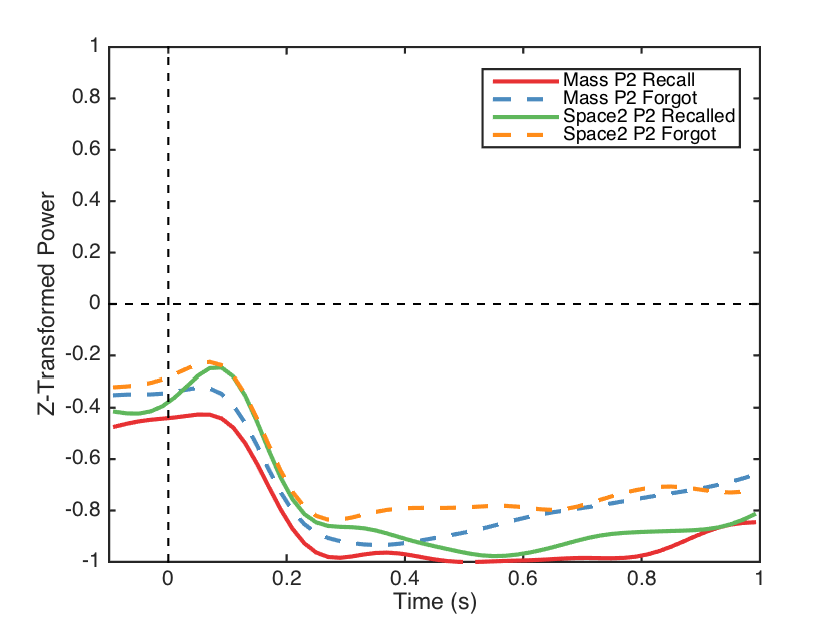
\includegraphics[width=.30\textwidth]{./figs/exp2/tfr_line/tfr_line_ga_img_rc_mass_p2_img_fo_mass_p2_img_rc_spac2_p2_img_fo_spac2_p2_11_12_-100_1000_44ROIs_legend} &
  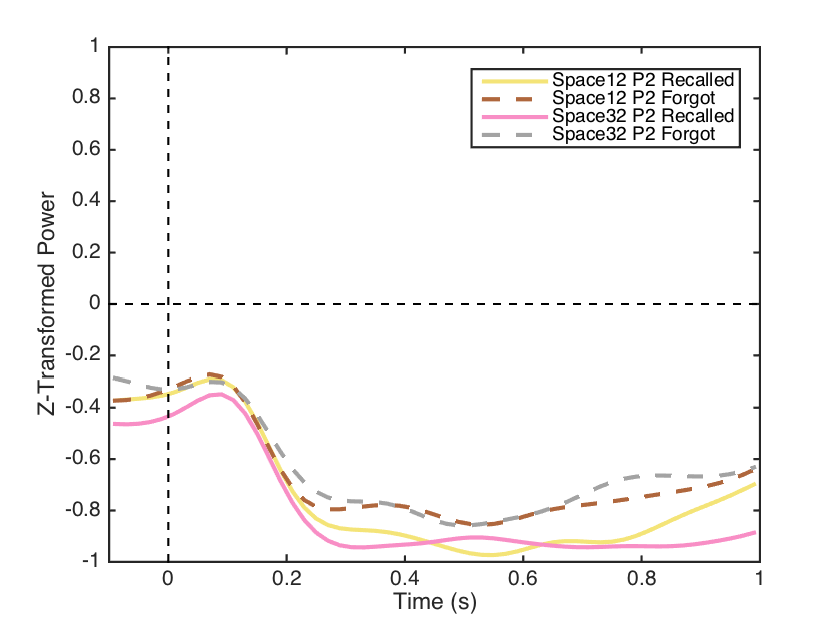
\includegraphics[width=.30\textwidth]{./figs/exp2/tfr_line/tfr_line_ga_img_rc_spac12_p2_img_fo_spac12_p2_img_rc_spac32_p2_img_fo_spac32_p2_11_12_-100_1000_44ROIs_legend} &
  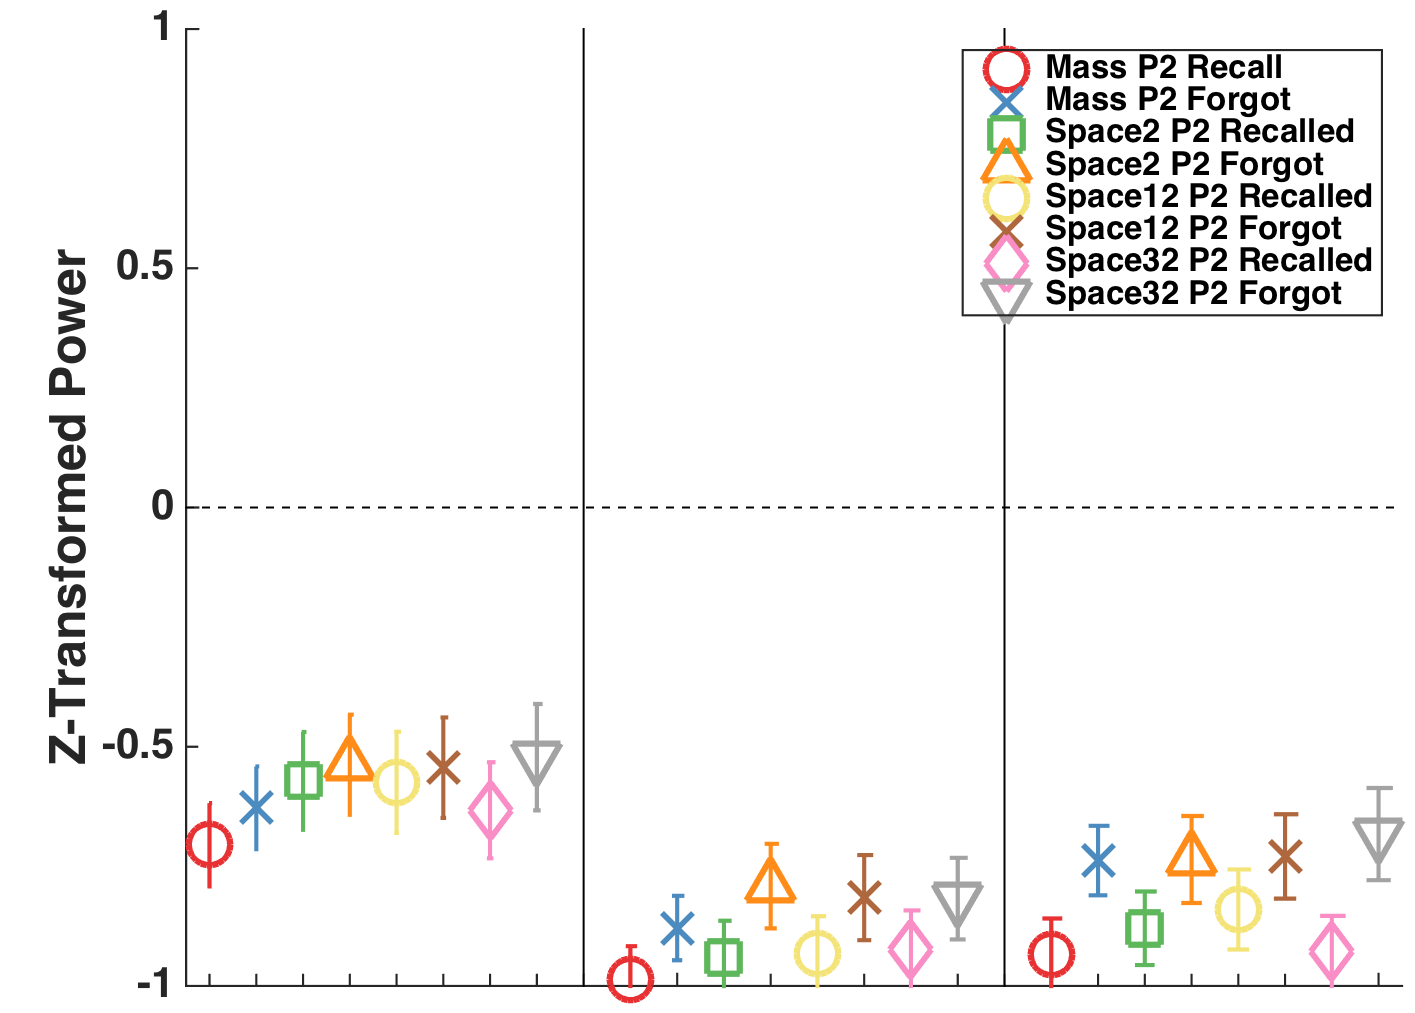
\includegraphics[width=.30\textwidth]{./figs/exp2/tfr_avg/tfr_avg_ga_img_rc_mass_p2_img_fo_mass_p2_img_rc_spac2_p2_img_fo_spac2_p2_img_rc_spac12_p2_img_fo_spac12_p2_img_rc_spac32_p2_img_fo_spac32_p2_11_12_0_333_333_666_666_1000_44ROI_ylabel} \\
  \end{tabular}
  \caption{Upper alpha to words and images.  (a), (b), (d), and (e) Grand averages; (c) and (f) mean values for the three time windows (error bars are SEM).}
  \label{fig:s2_word_img_alpha_upp}
  %Figure~\ref{fig:s2_word_img_alpha_upp}
\end{figure}

\textit{Word, upper alpha}: As in Experiment~1, we used three time windows for upper alpha and lower beta.  Across 46 electrodes (Figure~\ref{fig:s2_word_img_alpha_upp}, top), there was a main effect of time [$F(2,52)=18.3, p=2.36e^{-5}$]: the second and third time windows showed more upper alpha desynchronization than the first.  There was also a spacing $\times$ time interaction [$F(6,156)=11.8, p=9.2e^{-8}$]: each repetition decreased in power across time, but massed decreases more.

\textit{Image, upper alpha}: Across 44 electrodes (Figure~\ref{fig:s2_word_img_alpha_upp}, bottom), there were main effects of memory [$F(1,26)=21.8, p=8.08e^{-5}$] (recalled items desynchronized more than forgotten items) and time [$F(2,52)=25, p=3.55e^{-6}$]: power was lowest in the middle time window.  The spacing effect was marginally significant [$F(3,78)=2.74, p=.053$]: massed images desynchronized more than short and medium spaced items.  There was also a memory $\times$ time interaction [$F(2,52)=6.82, p<.005$] showing that the SME was strongest in the third time window.
% power for remembered items continued to desynchronize whereas power began to increse for forgotten items.


% plot: word and image lower beta
\begin{figure}[H]
  \centering
  \begin{tabular}{cccc}
  & Lower beta power & Lower beta power & Means \\
  & \multicolumn{1}{l}{(a)} & \multicolumn{1}{l}{(b)} & \multicolumn{1}{l}{(c)} \\
  \raisebox{1.8cm}{\rotatebox{90}{Word}} & 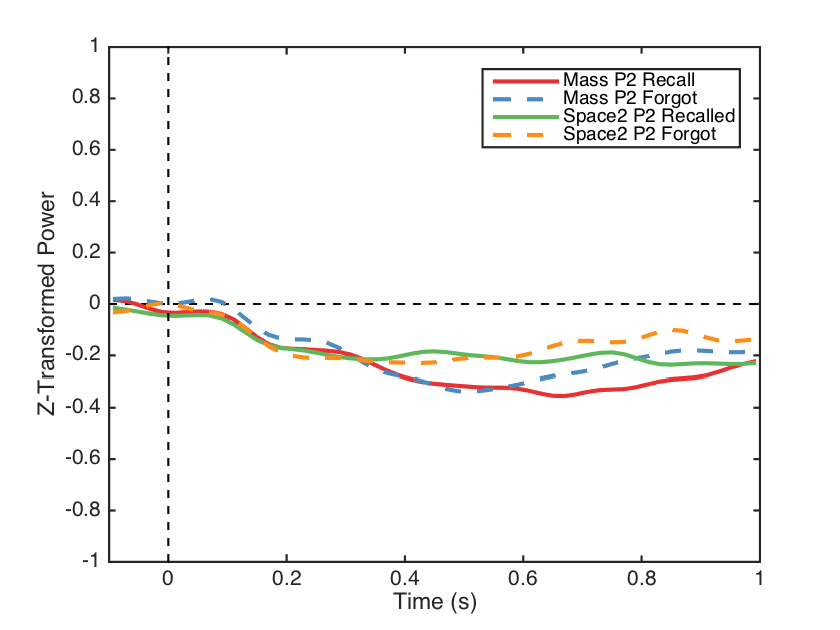
\includegraphics[width=.30\textwidth]{./figs/exp2/tfr_line/tfr_line_ga_word_rc_mass_p2_word_fo_mass_p2_word_rc_spac2_p2_word_fo_spac2_p2_13_21_-100_1000_66ROIs_legend} &
  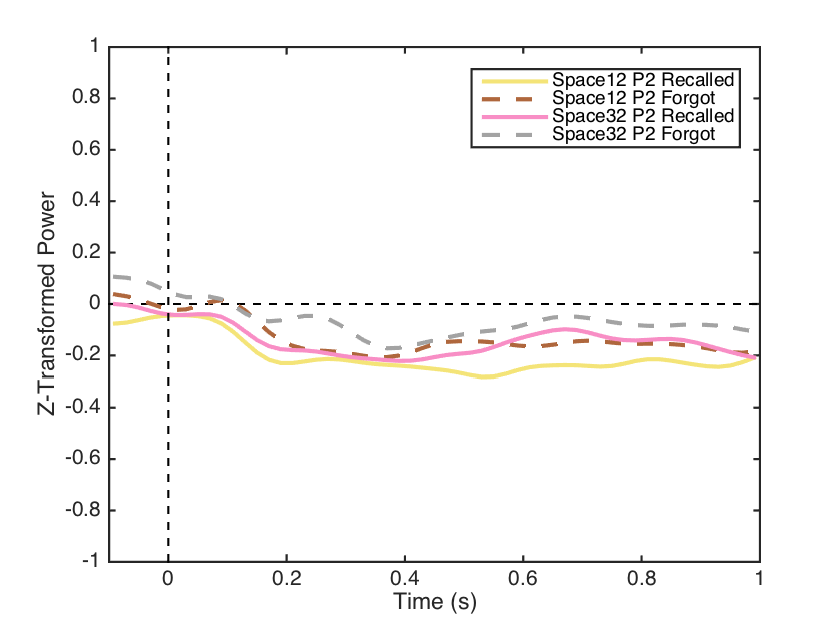
\includegraphics[width=.30\textwidth]{./figs/exp2/tfr_line/tfr_line_ga_word_rc_spac12_p2_word_fo_spac12_p2_word_rc_spac32_p2_word_fo_spac32_p2_13_21_-100_1000_66ROIs_legend} &
  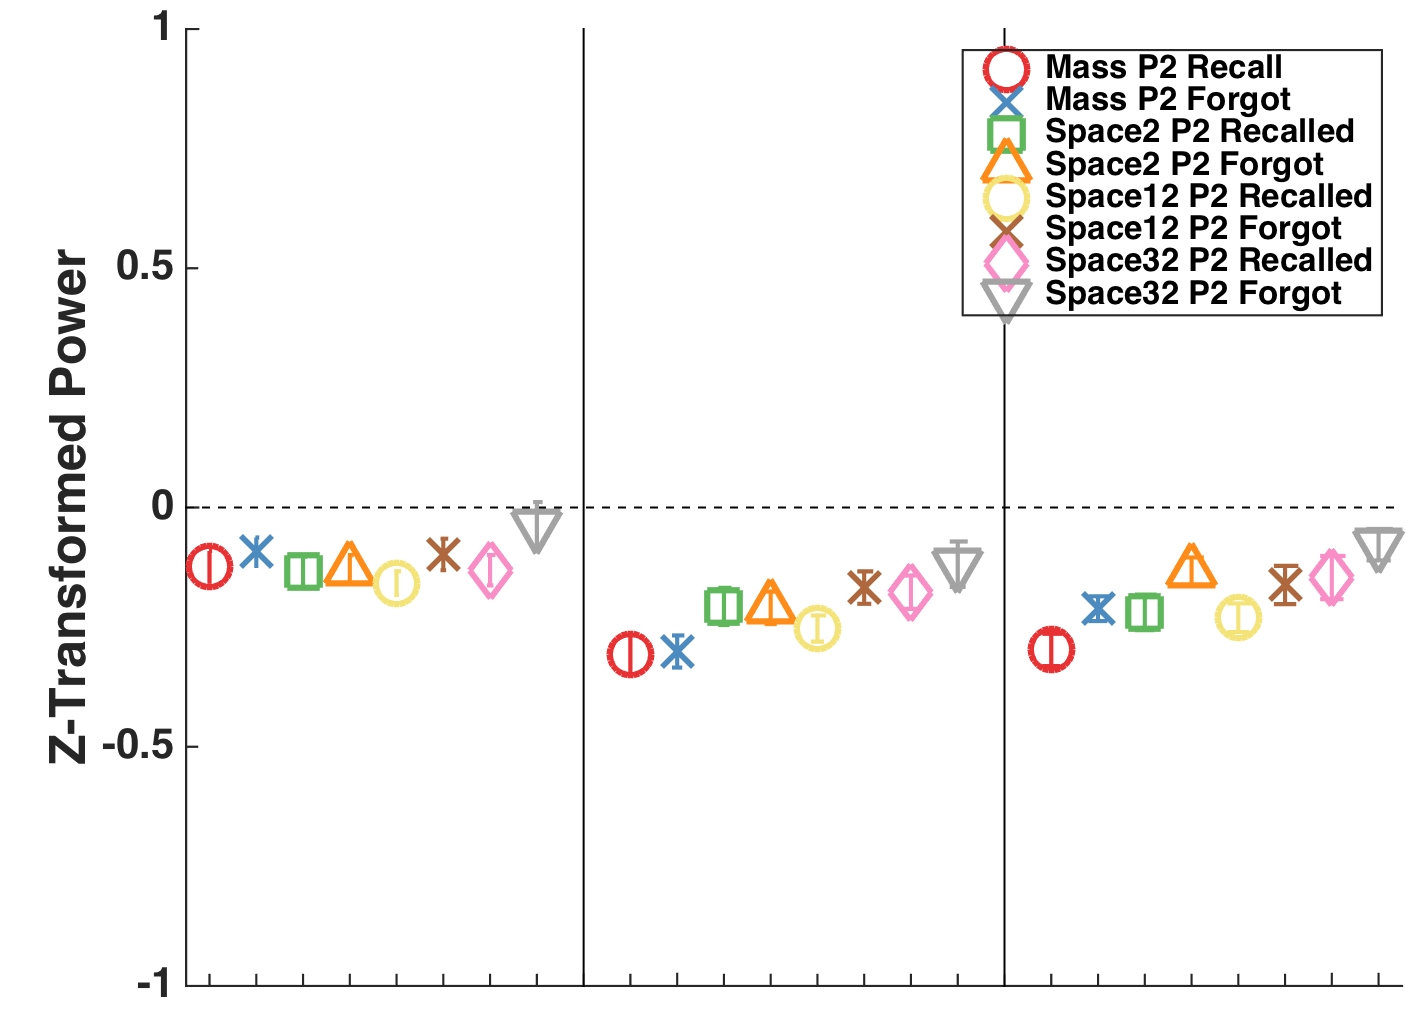
\includegraphics[width=.30\textwidth]{./figs/exp2/tfr_avg/tfr_avg_ga_word_rc_mass_p2_word_fo_mass_p2_word_rc_spac2_p2_word_fo_spac2_p2_word_rc_spac12_p2_word_fo_spac12_p2_word_rc_spac32_p2_word_fo_spac32_p2_13_21_0_333_333_666_666_1000_66ROI_ylabel} \\
  & \multicolumn{1}{l}{(d)} & \multicolumn{1}{l}{(e)} & \multicolumn{1}{l}{(f)} \\
  \raisebox{1.8cm}{\rotatebox{90}{Image}} & 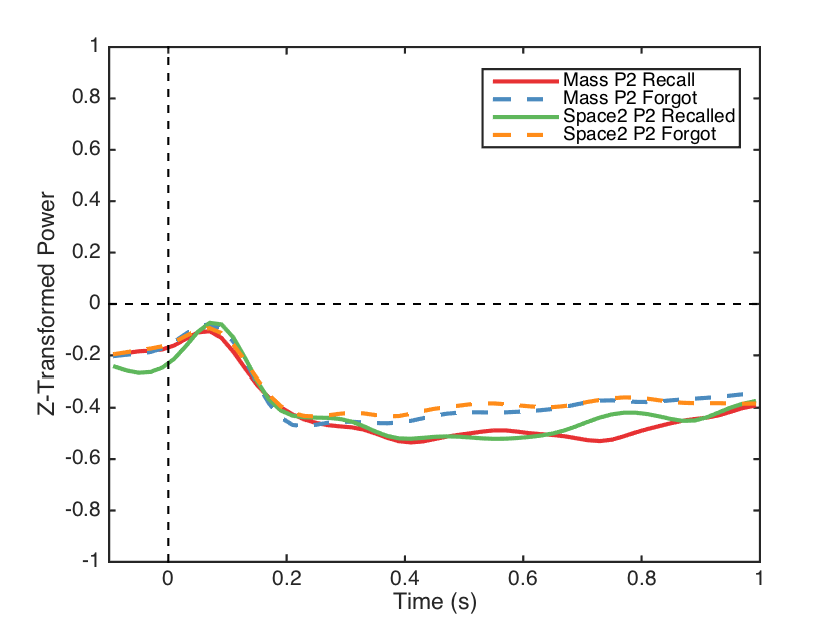
\includegraphics[width=.30\textwidth]{./figs/exp2/tfr_line/tfr_line_ga_img_rc_mass_p2_img_fo_mass_p2_img_rc_spac2_p2_img_fo_spac2_p2_13_21_-100_1000_30ROIs_legend} &
  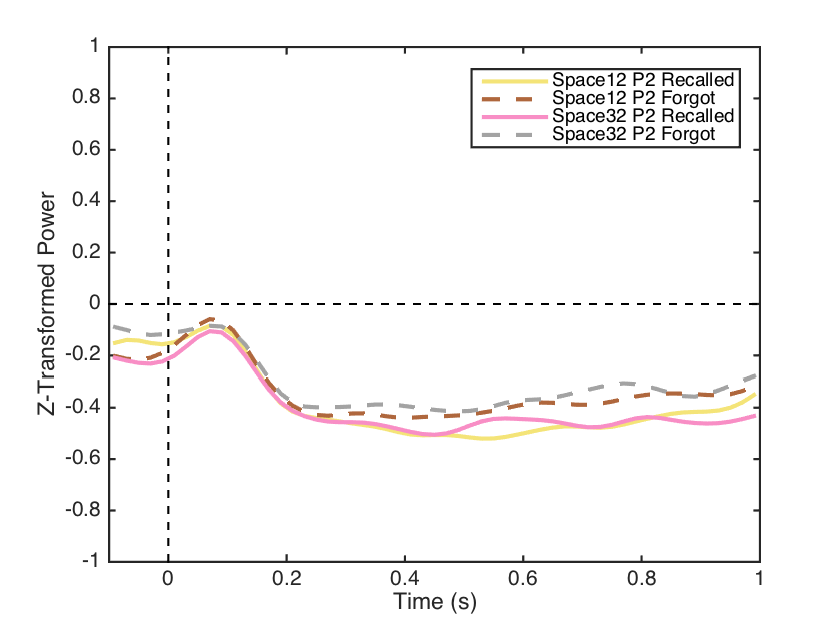
\includegraphics[width=.30\textwidth]{./figs/exp2/tfr_line/tfr_line_ga_img_rc_spac12_p2_img_fo_spac12_p2_img_rc_spac32_p2_img_fo_spac32_p2_13_21_-100_1000_30ROIs_legend} &
  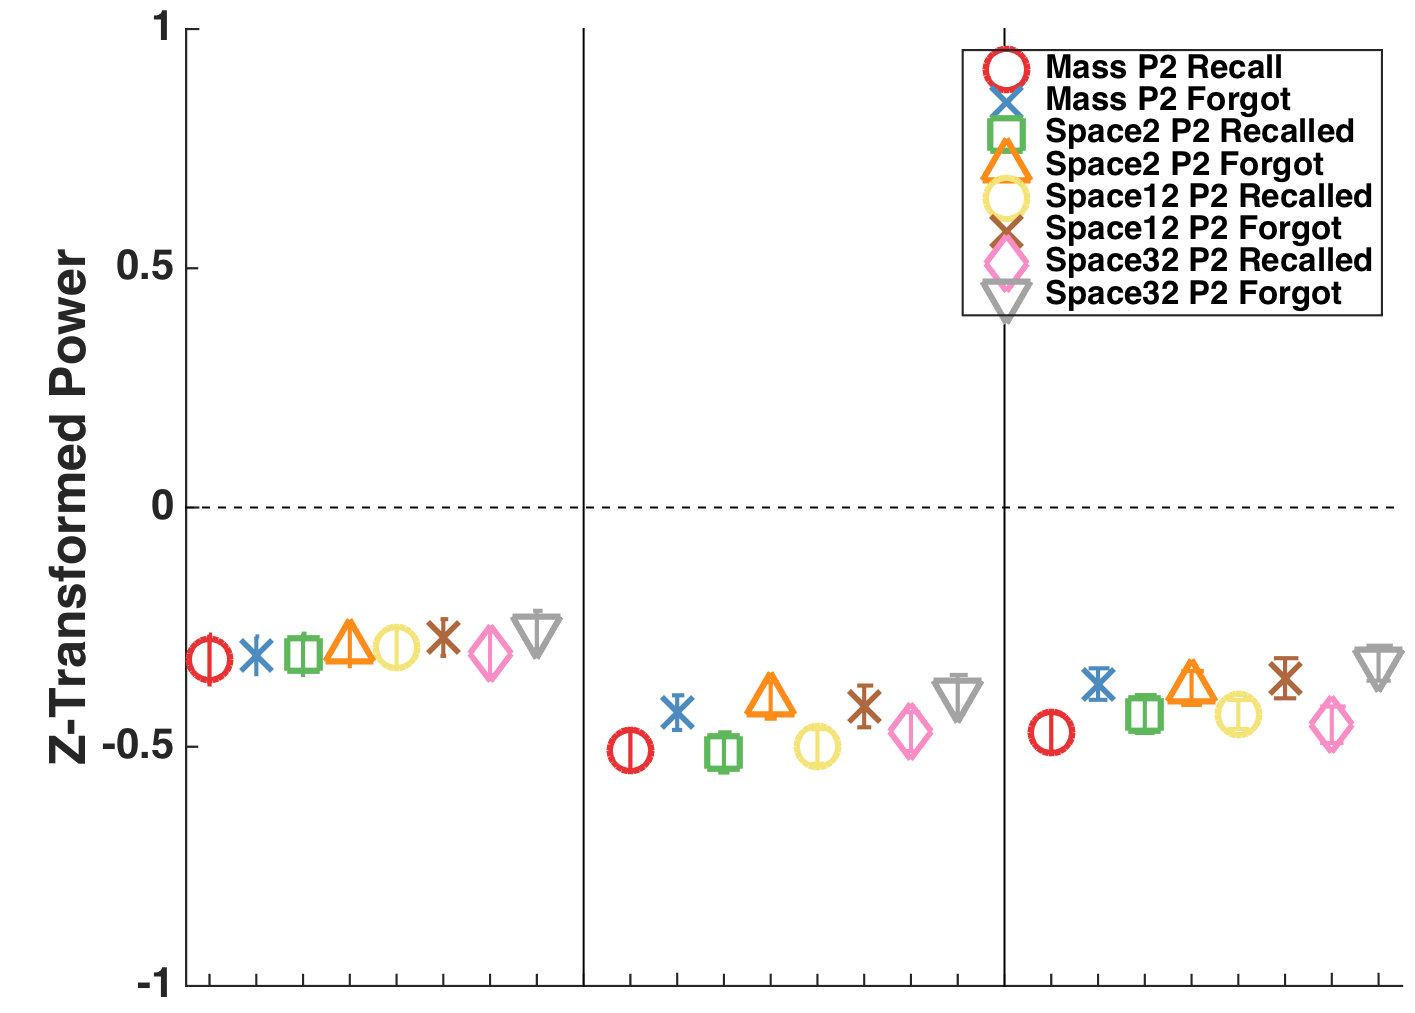
\includegraphics[width=.30\textwidth]{./figs/exp2/tfr_avg/tfr_avg_ga_img_rc_mass_p2_img_fo_mass_p2_img_rc_spac2_p2_img_fo_spac2_p2_img_rc_spac12_p2_img_fo_spac12_p2_img_rc_spac32_p2_img_fo_spac32_p2_13_21_0_333_333_666_666_1000_30ROI_ylabel} \\
  \end{tabular}
  \caption{Lower beta power to words and images.  (a), (b), (d), and (e) Grand averages; (c) and (f) mean values for the three time windows (error bars are SEM).}
  \label{fig:s2_word_img_beta_low}
  %Figure~\ref{fig:s2_word_img_beta_low}
\end{figure}


\textit{Word, lower beta}: Across 66 electrodes (Figure~\ref{fig:s2_word_img_beta_low}, top), there were main effects of spacing [$F(3,78)=9.48, p=7.16e^{-5}$], memory [$F(1,26)=8.36, p<.01$], time [$F(2,52)=25.5, p=5.06e^{-8}$], a spacing $\times$ time interaction [$F(6,156)=6.96, p=3.79e^{-6}$].
% and a marginal three-way interaction [$F(6,156)=2.02, p=.091$].
Massed word repetitions desynchronized more than the spaced conditions, subsequently recalled words desynchronized more than forgotten ones, and there was more desynchronization during the second time window compared to the others (though the third was still lower than the first).  Additionally, spacing effects across all spaced lags (short, medium, and long) were larger in the second and third time windows (massed were more negative).
%The marginal three-way interaction showed the same pattern as upper alpha: recalled items tended to stay desynchronized in the third time window while forgotten items increased slightly in power, and this increase seemed to happen more for short and long spaced items.


\textit{Image, lower beta}: Across 30 electrodes (Figure~\ref{fig:s2_word_img_beta_low}, bottom), there were main effects of memory [$F(1,26)=25.2, p=3.22e^{-5}$] and time [$F(2,52)=53.7, p=3.33e^{-12}$] which followed the patterns of effects reported above for words: recalled had more desynchronization, and power was lowest in the second time window and increased in the third.

\subsection{Time--frequency discussion}

%, and perhaps would also show stronger recollection memory ERP effects (such as the parietal old/new effect).}

% In addition to the LPC ERP voltage effect,
The theta band is a place where we expect to see effects of recollection and encoding,
%specifically in that subsequently remembered long-lag stimuli would show stronger reinstatement during repetitions.
especially at longer lags where retrieval would be more difficult but also more beneficial to long-term memory if successful
\cite{DelaEtal2010,PavlAnde2005}).
%\cite{Gree1989a}
Overall, the theta effects are quite similar to Experiment~1, and there is some variety across lags that is of interest for lag effects.
Theta power was sustained across word repetitions for spaced items compared to massed items, particularly for long (32) spaced words.  Recalled long (32) spaced words also showed higher power than all other conditions in the second time window.
This sustained theta spacing effect is interesting because these trials showed the highest behavioral memory performance.  In fact, the pattern of theta power across lags for recalled word repetitions in the second time window follows behavioral performance.  Thus, it seems that theta effects support study-phase retrieval in much the same was as Experiment~1, and theta may be an indicator of a lag effect.

For images, there was again a negative SME such that less theta power was associated with recalling the associated words during the test phase.  The discussion of this effect in Experiment~1 brought up the idea that it may be due to a more varied contextual state, though this again does not seem to mesh with the idea of little contextual drift occurring for massed repetitions.

% \hl{(Does it show a lag effect? Differences between lags?  Does theta power for each condition correlate with behavioral performance?)  The logic here is that theta is related to memory retrieval (and encoding/re-encoding); there should be strong retrieval for spaced items because they have left working memory, especially long (32) spaced items, and because the pattern of theta power for word repetitions follows behavioral performance, it seems possible that these are related (reverse inference).}

%If memory reinstatement occurs, we would expect to see effects in the theta band,   We would expect subsequently remembered long-lag stimuli to show a stronger reinstatement during repetitions.  This would manifest in the theta band.
% There was more theta power for long (32) spaced words compared to other conditions, including when only comparing those that were later recalled.  Since theta is related to memory reinstatement, this supports the idea that stronger retrieval occurred for these words compared to the other conditions.  This is in line with the idea that the more difficult retrieval is (due to increased spacing), given that retrieval occurs, the stronger the memory will be.


The lower alpha band generally correlates negatively with attentional processes and shows a widespread scalp topography.  Deficient processing would predict increased alpha power for massed repetitions, though the results for Experiment~1 were in the opposite direction (massed desynchronized more, or showed a decrease in power) and we expected these to be the same.  We also expected to see decreased power (more desynchronization) for better subsequent memory, due to increased attentional processing.
Lower alpha results followed Experiment~1: we see the memory effect just described, and the spacing effect again does not support deficient processing (more attention seems to get allocated to massed items).
%It is possible that these effects are affected by the contents of working memory.


For upper alpha,
%as with the N400 ERP component,
we expected semantic processing to show lag effects: remembered items should desynchronize more as lag increases because items with longer lag are remembered better on average, and semantic processing should help memory.  The results show that remembered items incur more semantic processing across the trial, but the spacing effect is opposite from what we predicted.  Massed items showed more semantic processing (and showed this earlier than spaced), so perhaps the effect is driven by the semantic representation being active in working memory.  As in Experiment~1, these results do not support deficient processing because it would predict less semantic processing for massed items.

The lower beta effects for words and images almost exactly follow those of Experiment~1.  This solidifies the idea that semantic processing (denoted by decreased power) helps memory overall.  Massed trials get a semantic processing boost during word presentations (more desynchronization in time windows 2 and 3), perhaps because they are in working memory, but spaced are equally processed during the images.

\subsection{Similarity results}

\begin{figure}[H]
  \centering
  %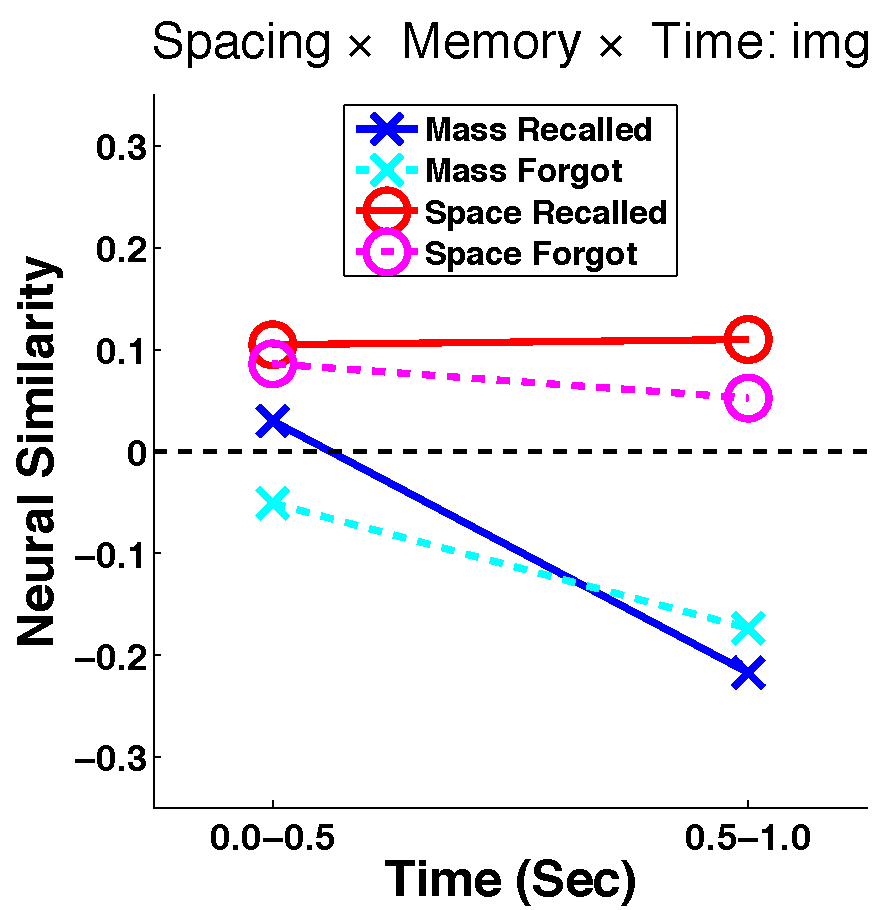
\includegraphics[width=.40\textwidth]{./figs/exp1/similarity_spacXmemXtime_img_tla_LTRT_0to500_500to1000_kaiser_cosine}
  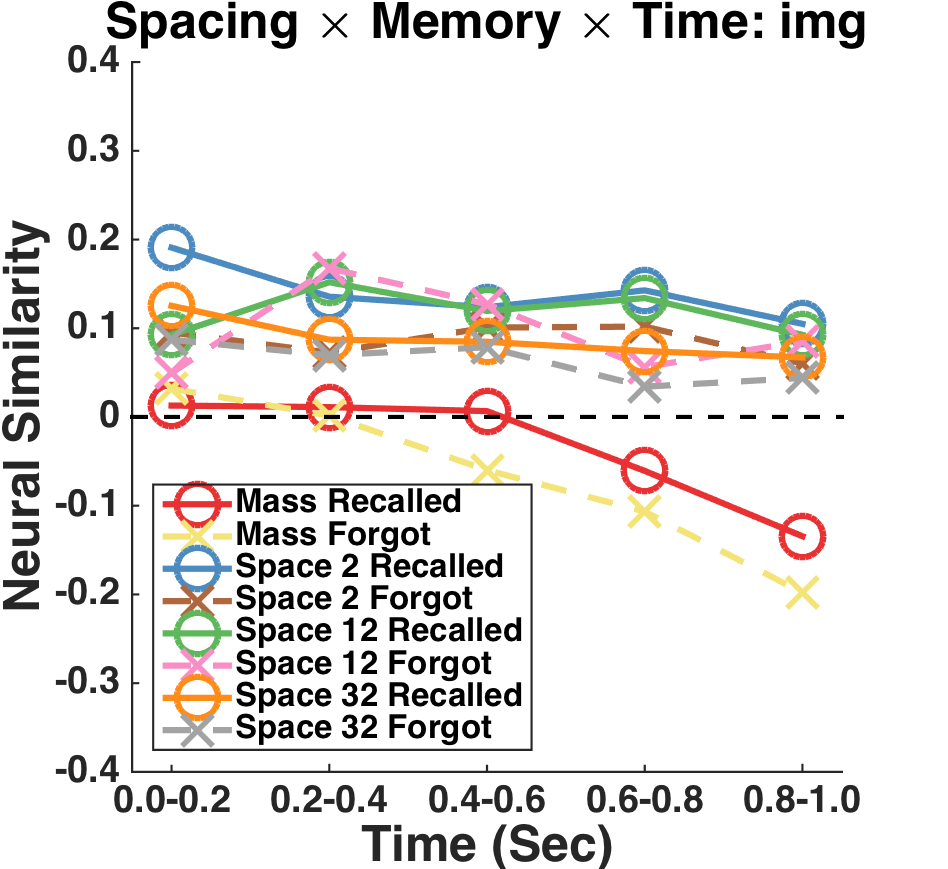
\includegraphics[width=.40\textwidth]{./figs/exp2/similarity_spacXmemXtime_img_tla_LTRT_0to200_200to400_400to600_600to800_800to1000_kaiser_cosine}
  \caption{Similarity for voltage at left and right temporal sites during image repetitions: Interaction between spacing, memory, and time [$n.s.$].}
  \label{fig:s2_sim_tla_spacXmemXtime}
  %Figure~\ref{fig:s2_sim_tla_spacXmemXtime}
\end{figure}

% \hl{Perhaps there is a way to select principal components that vary with memory performance and/or encoding strength.}  (Mentioned regarding \citeA{MannEtal2011} right before general discussion).

None of our effects for Experiment~2 have supported contextual variability; to do so, we would need to see more variability in EEG at as lag increases, an effect of temporocontextual drift.
% The closest effect this is related to in Experiment~1 results is in time--frequency similarity;
Perhaps a clearer picture will emerge with more lags.


The same ROIs, latencies, and data processing methods were used to measure neural similarity between initial and repetition trials as in Experiment~1, including using images for analysis because this is when word--image (item--context) binding should occur.
 

For voltage (Figure~\ref{fig:s2_sim_tla_spacXmemXtime}), a three-way repeated measures ANOVA was run on the average similarity values from left and right temporal regions with factors of spacing (spaced and massed), subsequent memory (recalled and not recalled), and time (successive 200~ms time bins).  There was a main effect of spacing [$F(3,78)=11.1, p=5.19e^{-6}$], a marginal effect of memory [$F(1,26)=3.92, p=.058$], and a main effect of time [$F(4,104)=6.31, p<.0005$].  There was also a spacing $\times$ time interaction [$F(12,312)=2.99, p=.005$].  Spaced items of all length lags were more similar than massed items, subsequently recalled items were marginally more similar than forgotten ones, and similarity decreased across time.  The interaction explains the two significant main effects in that massed item similarity decreased across time whereas spaced items stayed consistent.  These follow the results of Experiment~1, with the addition of the memory effect.

\begin{figure}[H]
  \centering
  %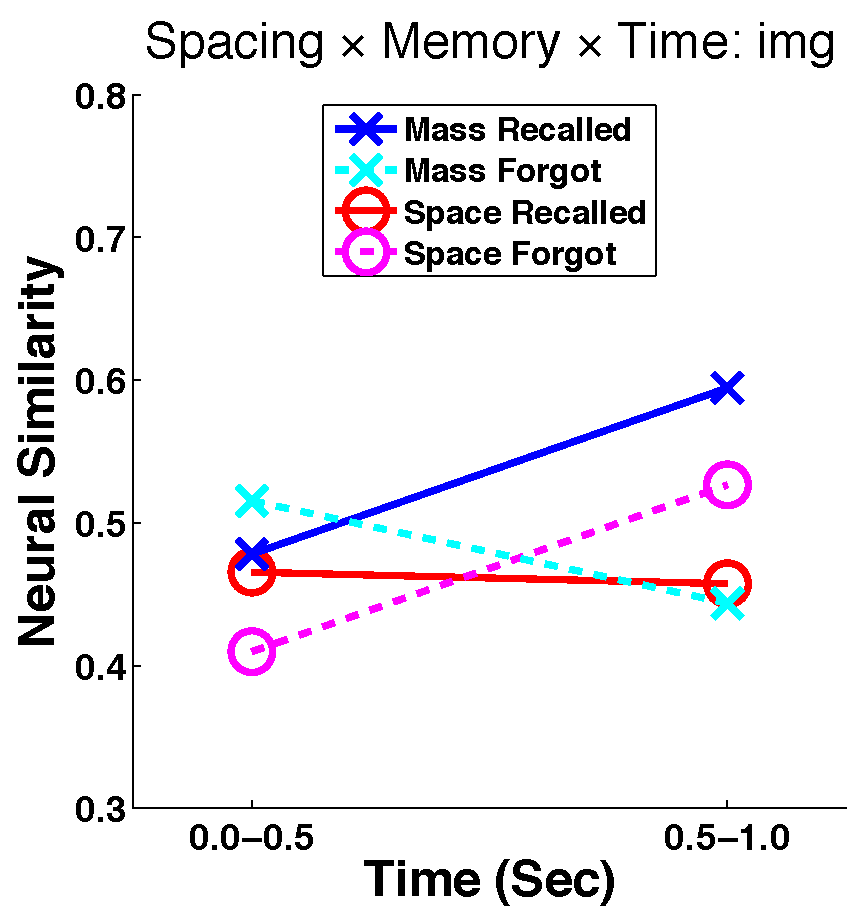
\includegraphics[width=.40\textwidth]{./figs/exp1/similarity_spacXmemXtime_img_pow_PS_0to500_500to1000_kaiser_cosine}
  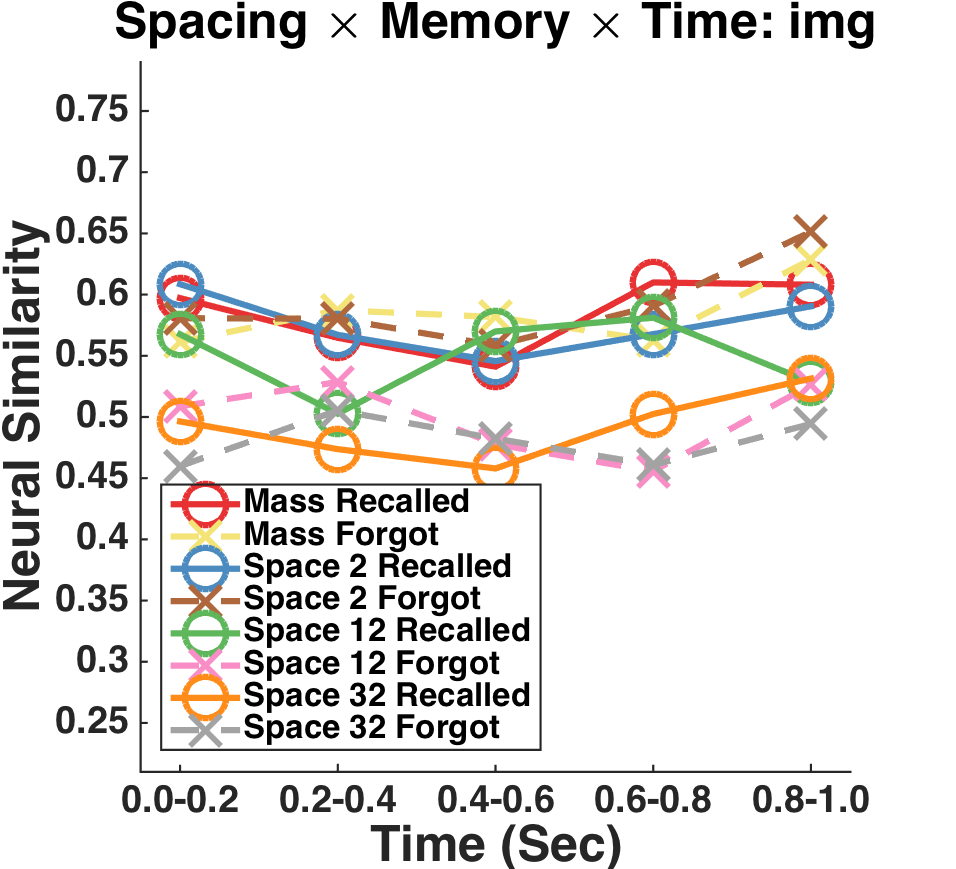
\includegraphics[width=.40\textwidth]{./figs/exp2/similarity_spacXmemXtime_img_pow_LPSRPS_0to200_200to400_400to600_600to800_800to1000_kaiser_cosine}
  \caption{Similarity for oscillatory power at left and right parietal sites during image repetitions: Interaction between spacing, memory, and time [$n.s.$].}
  \label{fig:s2_sim_pow_spacXmemXtime}
  %Figure~\ref{fig:s2_sim_pow_spacXmemXtime}
\end{figure}

For time--frequency data (Figure~\ref{fig:s2_sim_pow_spacXmemXtime}), the same three-way ANOVA was performed over left and right parietal regions across all frequency bands.
There was a main effect of spacing [$F(3,78)=8.92, p=6.5e^{-5}$] (similarity decreased with lag), a main effect of time [$F(4,104)=2.9, p<.05$] (similarity increased across time), and a marginal memory $\times$ time interaction [$F(4,104)=2.46, p=0.051$] (without a clear pattern).  These also follow the results of Experiment~1, though the interaction was less clear here.

\subsection{Similarity discussion}

The patterns for voltage and time--frequency data mimicked Experiment~1 in the same way.  Repeating some of the discussion from the prior experiment, it seems that for voltage, spaced repetitions tend to induce a consistent representation across time (possibly supporting study-phase retrieval) while massed repetitions become more variable.  This could be attributed to noise being is added to the system (supporting deficient processing), inducing a more variable representation (supporting contextual variability), or engaging different neural/cognitive processes.  It does not seem like noise would be added to the system when a massed stimulus received semantic processing at the repetition (earlier upper alpha and lower beta results), and from a theoretical standpoint there is no good reason for massed repetitions to have more variable representations because context has not drifted.  Study-phase retrieval seems like the most reasonable explanation for the advantage for spaced items (the spacing effect) at this point.

%, and perhaps massed items are being processed or thought about differently during the repetition.

% Another way to support deficient processing is if the first massed presentation received full attentional processing and the repetition is processed deficiently

\section{Experiment~2 discussion}

\cbstart
The purpose of this experiment was to look for lag effects in relation to neural activity to better interpret data patterns in the context of the three theories.
Behaviorally, we saw exactly what was expected: performance increased significantly as lag increased.  The EEG effects mostly followed the patterns of Experiment~1.  Across the ERP results, it seems like information that is already in working memory and does not need to be retrieved (massed) does not gain the repetition advantage of information that needs to be retrieved (spaced).

For many effects there was no difference between spaced condition lags, which was not what we were hoping for.  However, increased theta power is associated with memory retrieval, and it varied positively with repetition lag (as spacing increased).  Additionally, in the voltage similarity analysis, a more similar neural state during the repetition (compared to the initial presentation) leads to better subsequent memory.   Overall, the spacing effect seems to be more consistently driven by retrieval of a prior occurrence than by any other process, and therefore it seems that study-phase retrieval is a key part of the spacing effect.
\cbend

% No difference between spaced: N1, N400, LPC
% Diff bt spaced: LPC latency, theta


%Deficient processing is supported by:
%N1: a weak decrease in attention for massed items.

% It is interesting to contrast increased theta for long spaced items with the LPC effects where massed items showed the most retrieval.  As was mentioned before, the LPC in this task may be related to information in working memory and may not necessarily reflect recollection.
